
\documentclass[12pt,oneside]{article}

%%%%%%%%%%%%%%%%%%%%%%%%%%%%
%%   Zusaetzliche Pakete  %%
%%%%%%%%%%%%%%%%%%%%%%%%%%%%
\usepackage{enumerate}  
\usepackage{fancyhdr}
\usepackage{polynom}
\usepackage{a4wide}
\usepackage[utf8]{inputenc}
\usepackage{graphicx}
\usepackage{palatino}
\usepackage{python}
\usepackage{scrextend}
\usepackage{multirow}
\usepackage[toc,page]{appendix}
\usepackage{booktabs}
\usepackage{listings}
\usepackage{titlesec}
\usepackage{amsthm}
\usepackage{amssymb}
\usepackage{amsmath}
\usepackage[utf8]{inputenc}
\usepackage[options ]{algorithm2e}
\usepackage[ruled,vlined]{algorithm2e}
\usepackage{lmodern}
\usepackage[utf8]{inputenc}
\usepackage[english,german]{babel}
\usepackage{xcolor}
\usepackage{amsfonts}
\usepackage{etoolbox}
\usepackage[]{algorithm2e}
\usepackage{blindtext}
\usepackage{algorithm}
\usepackage[noend]{algpseudocode}
\usepackage{comment}
\usepackage[
backend=biber,
style=alphabetic,
sorting=ynt
]{biblatex}
\usepackage{enumitem}% http://ctan.org/pkg/enumitem

% for footnotes
\deffootnote[10pt]{10pt}{10pt}{\makebox[10pt][l]{\thefootnotemark\hspace{10pt}}}

% notendig für Definitionen und Theoreme
\newtheorem{theorem}{Theorem}[section]
\newtheorem{corollary}{Corollary}[theorem]
\newtheorem{lemma}[theorem]{Lemma}
\newtheorem{fact}[theorem]{Fakt}
\newtheorem{example}[theorem]{Beispiel}
\newtheorem{conj}[theorem]{Vermutung}
\newtheorem{question}[theorem]{Frage}

\newtheorem{prop}{Proposition}[section]

\theoremstyle{remark}
\newtheorem*{remark}{Remark}

\theoremstyle{definition}
\newtheorem{definition}{Definition}[section]
%%%%%%%%%%%%%%%%%%%%%%%%%%%%%%

%folgende Zeile auskommentieren für englische Arbeiten
\usepackage[ngerman]{babel}
%folgende Zeile auskommentieren für deutsche Arbeiten
%\usepackage[ngerman, english]{babel}
\usepackage[T1]{fontenc}
\usepackage[utf8]{inputenc}
\usepackage[bookmarks]{hyperref}
\usepackage[justification=centering]{caption}
\usepackage[style=authoryear,natbib=true,backend=biber,maxbibnames=20]{biblatex}
\usepackage{csquotes}
\bibliography{literatur}
\addbibresource{literatur.bib}
\setlength{\parindent}{0em} 
\setlist[itemize]{noitemsep, topsep=0pt}
\setlist[enumerate]{noitemsep, topsep=0pt}


%%%%%%%%%%%%%%%%%%%%%%%%%%%%%%
%% Definition der Kopfzeile %%
%%%%%%%%%%%%%%%%%%%%%%%%%%%%%%

\pagestyle{fancy}
\fancyhf{}
\cfoot{\thepage}
\setlength{\headheight}{16pt}
\newcommand\showdiv[1]{\overline{\smash{)}#1}}
%%%%%%%%%%%%%%%%%%%%%%%%%%%%%%%%%%%%%%%%%%%%%%%%%%%%%
%%  Definition des Deckblattes und der Titelseite  %%
%%%%%%%%%%%%%%%%%%%%%%%%%%%%%%%%%%%%%%%%%%%%%%%%%%%%%

\newcommand{\JMUTitle}[9]{

  \thispagestyle{empty}
  \vspace*{\stretch{1}}
  {\parindent0cm
  \rule{\linewidth}{.7ex}}
  \begin{flushright}
    \vspace*{\stretch{1}}
    \sffamily\bfseries\Huge
    #1\\
    \vspace*{\stretch{1}}
    \sffamily\bfseries\large
    #2\\
    \vspace*{\stretch{1}}
    \sffamily\bfseries\small
    #3
  \end{flushright}
  \rule{\linewidth}{.7ex}

  \vspace*{\stretch{1}}
  \begin{center}
    
\includegraphics[width=4in]{logo} \\
    \vspace*{\stretch{1}}
    \Large  Bachelorarbeit   \\

    \vspace*{\stretch{2}}
   \large Lehrstuhl für Mathematik \\
    \large und Informatik \\
    \large Universität Leipzig\\
    \vspace*{\stretch{1}}
    \large Betreuer:  #8 \\[1mm]
    
    \vspace*{\stretch{1}}
    \large Leipzig, den #7
  \end{center}
}

\titlespacing*{\section}
{0pt}{3.5ex plus 1ex minus .2ex}{.2ex plus .2ex}
\titlespacing*{\subsection}
{0pt}{1.5ex plus 1ex minus .2ex}{.2ex plus .2ex}
\titlespacing*{\subsubsection}
{0pt}{1.5ex plus 1ex minus .2ex}{.2ex plus .2ex}

%%%%%%%%%%%%%%%%%%%%%%%%%%%%
%%  Beginn des Dokuments  %%
%%%%%%%%%%%%%%%%%%%%%%%%%%%%

\begin{document}

  \JMUTitle
      {Deterministischer Primzahltest mit polynomieller Laufzeit: Der AKS-Primzahltest}  
      {Salman Salman}                        
      {3753924}
      
      {Fakultät für Informatik und Mathematik}  % Name der Fakultaet
      {Leipzig 2020}                          % Ort und Jahr der Erstellung
      {\today}                              % Tag der Abgabe
      {Prof. Dr. Andreas Maletti}               % Name des Erstgutachters
      {Zweitgutachter}                          % Name des Zweitgutachters
      
  \clearpage

\lhead{}
\pagenumbering{Roman} 
    \setcounter{page}{1}

\tableofcontents
\clearpage

\addcontentsline{toc}{section}{\listfigurename}
\listoffigures

\addcontentsline{toc}{section}{\listtablename}
\listoftables
\clearpage

\setlength{\parskip}{0.5em} 


%%%%%%%%%%%%%%%%%%%%%%%%%%%%
%%  Kurzzusammenfassung   %%
%%%%%%%%%%%%%%%%%%%%%%%%%%%%
\lhead{Abstract}
\section*{Abstract}
Primzahlen haben in der Informatik, speziell im Anwendungsgebiet der Kryptographie, eine sehr hohe Relevanz für moderne kryptographische Systeme ist es von Wichtigkeit selbige schnell bestimmen zu können. Hierzu werden effiziente Algorithmen zur Lösung des Primalitätsproblems(PRIMES) benötigt. Das Primalitätsproblem umfasst die Frage um die Entscheidung, ob eine gegebene Zahl eine Primzahl ist oder nicht. Der erste deterministische Primzahltest in Polynomialzeit wurde von den indischen Informatikern Agrawal, Kayal, und Saxena vorgestellt. Der nach ihnen benannte AKS-Primzahltest wird im Rahmen dieser Arbeit repräsentiert, implementiert und evaluiert.  


%%%%%%%%%%%%%%%%%%%%%%%%%%%%
%%  Einstellungen  %%
%%%%%%%%%%%%%%%%%%%%%%%%%%%%
\clearpage
\pagenumbering{arabic}  
    \setcounter{page}{1}
\lhead{\nouppercase{\leftmark}}

%%%%%%%%%%%%%%%%%%%%%%%%%%%%
%%  Hauptteil  %%
%%%%%%%%%%%%%%%%%%%%%%%%%%%%

 

\section{Einleitung} \label{einleitung}

\subsection{Gliederung der Arbeit}
Die Arbeit gliedert sich in sechs Bestandteile, wobei der
erste Teil die Einleitung darstellt. Dort wird ein Überblick in das Thema gegeben und die Zielsetzung der Arbeit definiert.

Das zweite Kapitel enthält die Grundlagen. Hier werden Begriffe und Konzepte erläutert, die für das weitere Verständnis der Arbeit eine Rolle spielen. 

Der Algorithmus und seine Korrektheit sind die Bestandteile des dritten Kapitels. Dort wird zunächst die Grundidee des AKS-Algorithmus erläutert. Danach wird der Algorithmus angegeben, dabei werden die Schritte des Algorithmus auch erklärt. Anschließend soll die Korrektheit des Algorithmus bewiesen. 

Im vierten Kapitel wird die mathematische Laufzeitanalyse des AKS-Algorithmus vorgestellt, dabei werden die Laufzeiten der einzelnen Schritte (STEPS 1-6) des AKS-Algorithmus ausführlich analysiert. Anschließend werden mögliche Verbesserungen der Laufzeit vorgestellt. 

Das fünfte Kapitel beinhaltet die experimentelle Laufzeit- und Korrektheitsanalyse, dort  soll die Laufzeit der Schritte des AKS-Algorithmus auf einem Rechner getestet werden. Darüber hinaus soll auch die Korrektheit dieser Schritte geprüft werden. Schließlich soll der AKS-Algorithmus mit dem naiven Algorithmus\footnote{. Der naive Algorithmus ist der beste nicht probabilistische Algorithmus. Die Laufzeit dieses Algorithmus ist $\Omega(\sqrt{n})$} verglichen werden.


\subsection{Überblick}
Eine Primzahl ist eine von 1 verschiedene natürliche Zahl, die keine Teiler außer 1 und sich selbst hat. Die Frage, ob eine Zahl eine Primzahl ist oder nicht, war schon im antiken Griechenland interessant. Euklid hat sich mit dieser Frage beschäftigt und bewiesen, dass es unendlich viele Primzahlen gibt. Im 3. Jahrhundert v. Chr. hat der griechische Mathematiker Eratosthenes einen Algorithmus zur Bestimmung einer Liste aller Primzahlen kleiner oder gleich einer vorgegebenen Zahl vorgestellt. Sein Algorithmus ist jedoch zur Lösung des Primalitätsproblem nicht effizient, da die Generierung solcher Listen bei sehr großen Zahlen extrem aufwendig wird.

Im 17. und 18. Jahrhundert haben Wissenschaftler nach einem Verfahren zum Finden von Primzahlen gesucht. Ein wichtiges Resultat war der Satz von Wilson, der britische Mathematiker John Wilson(1741-1793) hat einen Satz formuliert, um Primzahlen von zusammengesetzten Zahlen zu unterscheiden. Der Satz lautet: $p \geq 2$ ist genau dann eine Primzahl, wenn $(p - 1)! + 1$ durch $p$ teilbar ist. Der französische Wissenschaftler Marin Mersenne(1588 - 1648) hat sich auch mit Primzahlen beschäftigt, er behauptete, dass für eine nach ihm benannte mersennsche Zahl(eine Zahl der Form $2^p - 1$) genau dann eine Primzahl, wenn $p$ eine Primzahl ist. Seine Behauptung war jedoch nicht vollständig\footnote{$p = 67$ ist prim aber $2^{67} - 1 = 0 \, mod \, \, 193707721$}, beispielsweise $ p = 67 \in \mathbb{P}$, aber $2^{67} - 1 \not \in \mathbb{P}$. Obwohl diese Behauptung falsch war, hat sie sehr viel zur mathematischen Theoriebildung beigetragen. Zahlen für die $2^p - 1 \in \mathbb{P}$ gilt, heißen mersennsche Primzahlen. Die größte Primzahl heute(Jahr: 2020) $2^{82,589,933}$ $ - 1$ ist eine mersennsche Primzahl\cite{largePrimes}. Ein anderer französischer Mathematiker Pierre de Fermat(1607-1665) hat einen Satz zur Beschreibung der Eigenschaften von Primzahlen aufgestellt. Sein Satz ist später die Grundlage für Primzahltests geworden.
\newline

Die Sätze(Algorithmen) von Wilson, Mersenne, und Fermat sind aber zum Finden von großen Primzahlen nicht geeignet und ineffizient. Natürlich hat damals sowieso niemand versucht, große Primzahlen mittels dieser Sätze zu finden, da es einfach keinen Grund dafür gab. Der frühste Einsatz von großen Primzahl findet sich im 20. Jahrhundert bei modernen kryptographische Systemen\cite{krypWiki}. Im Jahr 1997 wurde mit dem RSA-Verfahren eine Methode entdeckt, mit der man Daten sehr sicher verschlüsseln kann und die auch für den allgemeinen Gebrauch geeignet ist. Bei diesem verfahren muss aber ein Produkt aus Primzahlen berechnet werden\cite{rsa}. Man beachte dabei, dass die in der Praxis eingesetzte Primzahlen sehr groß sind und aus mehreren Hundert Stellen bestehen können. Aus diesem Grund ist es sinnvoll einen Algorithmus(oder mehrere Algorithmen) zu haben, mit dem man solche Primzahlen \textquotedbl schnell\textquotedbl   $\;$ bestimmen kann. Um das zu verwirklichen, braucht man zunächst eine formale Definition vom untersuchten Problem und darüber hinaus eine Definition für schnelle Algorithmen. Hier kommen die Komplexitätstheorie und die Berechenbarkeitstheorie zum Einsatz. 

Seit dem Beginn der Komplexitätstheorie in den 1960er Jahren, wurden Begriffe formalisiert und verschiedene Komplexitätsklassen definiert\cite{com-theory}. Seitdem versuchten Informatiker und Mathematiker, das Primalitätsproblem in einer Komplexitätsklasse einzuordnen. Daher wurde das Primalitätsproblem auch im Laufe der Jahre intensiv untersucht. Es war trivial zu sehen, dass dieses Problem in der Komplexitätsklasse co-NP liegt\footnote{Dies entspricht der Aussage, dass geprüft wird, ob eine Zahl $n$ zusammengesetzt ist in NP. Man soll hier nun ein Zertifikat (Faktor) $d$ finden und testen ob $d \mid n$ gilt. Dies ist offensichtlich in Polynomialzeit realisierbar.}. In 1974 hat der australische Informatiker Vaughan Pratt eine wichtige Beobachtung gemacht, nämlich, dass das Primalitätsproblem auch in der Komplexitätsklasse NP liegt\cite{pratt}.

Die Frage war nachher zu klären, ob das Primalitätsproblem auch in P liegt. Mit anderen Worten, dass es einen Algorithmus(Primzahltest) mit polynomieller Laufzeit gibt und das Primalitätsproblem löst. Viele Wissenschaftler haben danach versucht, auf diese Frage zu beantworten, dazu wurden zahlreiche Primzahltests entwickelt. Leider war keiner der Versuche erfolgreich, da alle entwickelten Primzahltests entweder von unbewiesenen Hypothesen, wie zum Beispiel die verallgemeinerte Riemannsche Vermutung, abhängig waren oder probabilistisch waren\footnote{Probabilistische Algorithmen sind randomisierte Algorithmen, die auch ein falsches Ergebnis liefern können(nicht deterministisch)}. Ein bekannter probabilistischer Primzahltest ist der Miller-Rabin-Primzahltest, er kann das Primalitätsproblem in $O(k log^3 n)$ lösen\cite{milRab}. Allerdings kann der beste nicht probabilistische Algorithmus (bis 2002) das Primalitätsproblem in $ \Omega(\sqrt{n}) $ Schritten lösen, wobei $n$ die Eingabegröße ist(Die Eingabe ist in diesem Fall die Anzahl der nötigen Bits, um die Zahl $n$ zu repräsentieren). Dieser Primzahltest heiß der Probedivision-Primzahltest oder naiver Primzahltest und hat eine exponentielle Zeit.\footnote{Für eine Erklärung, warum ein Algorithmus mit $\Omega(\sqrt{n})$ im Rahmen von Primalitätstesten eine exponentielle Laufzeit hat siehe: \url{https://cs.stackexchange.com/questions/88398/primality-testing-why-is-dividing-a-number-n-by-every-integer-between-2-and}.} In 2002 haben drei Informatiker Agrawal, Kayal, und Saxena den ersten deterministischen unbedingten Algorithmus vorgestellt, der das Primalitätsproblem in polynomiellzeit lösen kann. Das heißt sie haben gezeigt, dass das Primalitätsproblem(PRIMES) zur Komplexitätsklasse $P$ gehört.      

\subsection{Zielsetzung}
Im dieser Arbeit wird der AKS-Primzahltest aus dem Originalartikel(\cite{aks}) behandelt. Ziel dieser Arbeit ist die Korrektheit des AKS-Algorithmus zu demonstrieren und seine Laufzeit zu evaluieren. Um die Korrektheit zu zeigen soll Zunächst der mathematische Korrektheitsbeweis durchgeführt. Neben dem mathematischen Beweis werden auch mehrere Tests durchgeführt, um die Korrektheit experimentell zu beweisen. Die Ergebnisse dieser Tests werden mittels Tabellen sowie Grafiken dargestellt. Dazu wird der Algorithmus auf einem Rechner implementiert und durch mehrere Testfälle evaluiert. Der AKS-Algorithmus ist hauptsächlich dafür bekannt, das Primalitätsproblem in Polynomialzeit zu lösen, diese Eigenschaft wird auch untersucht. Hier wird auch auf ähnlicher Weise erst mathematisch und dann experimentell bewiesen, dass der AKS-Algorithmus eine polynomielle Laufzeit hat. Schließlich soll der AKS-Algorithmus mit dem naiven Primzahltest verglichen.  


\newpage


\section{Grundlagen}
In diesem Kapitel handelt es sich darum, die essenziellen Begriffe und Theoreme aus der Zahlentheorie, der Algebra und der Komplexitätstheorie, die für den AKS-Algorithmus relevant sind, zu definieren.
% Definitionen der Zhalentheorie 
% Definitonen

\smallskip

% Zahlentheorie

\subsection{Zahlentheorie}
In diesem Abschnitt werden grundlegende Begriffe und Theoreme aus der Zahlentheorie definiert(und ggf. bewiesen). Zuerst werden zahlentheoretische Funktionen und Begriffe definiert. Des Weiteren werden Theoreme, die für das Verständnis des AKS-Algorithmus erforderlich sind, dargestellt und bewiesen. Beispielsweise, die Sätze von Euler und Fermat. Hier wird angenommen, das der Leser eine rudimentäre Kenntnisse über die Zahlentheorie hat. Für eine ausführliche Einführung in die Zahlentheorie und Primzahlen siehe \cite{prime-numbers}.\newline

\theoremstyle{definition}
\begin{definition}\label{Df_1}
Seien $a,b \in \mathbb{N}$. Der \textbf{größte gemeinsame Teiler} von $a$ und $b$ wird mit $(a,b)$ bezeichnet, ist die größte positive Zahl $n$, sodass $n \mid a$ und $n$ $ \mid b$
\end{definition}

\smallskip

\begin{theorem}
Seien $a,b \in \mathbb{N}$, dann existieren $x,y \in \mathbb{N}$, sodass $(a,b) = ax + by$ 
\end{theorem}

\smallskip

\begin{definition}\label{Df_2}
Zwei Zahlen $a,b \in \mathbb{N}$ heißen genau dann \textbf{Teilerfremd}, wenn $(a,b) = 1$.
\end{definition}

\begin{example}
Der größte gemeinsame Teiler von $24,16$ ist $(24,18) = 6$, für zwei teilerfremde Zahlen wie $5,9$ gilt $(5,9) = 1$. 
\end{example}

\smallskip 



\smallskip

\begin{definition}
Seien $n, m$ zwei natürliche Zahlen, dann heißt die kleinste positive natürliche Zahl, die sowohl ein Vielfaches von $n$, als auch von $m$ \textbf{kleinstes gemeinsames Vielfaches} beider zahlen. Hier wird das kleinste gemeinsame Vielfaches mit \textbf{kgV} bezeichnet.
\end{definition}

\smallskip

\begin{definition}\label{Df_5}
Sei $n \in \mathbb{N}$, die \textbf{Primzahlzerlegung} von $n$ ist die Darstellung der Zahl als Produkt ihrer Primfaktoren \newline
\begin{equation}
    n = p_{1}^{e_{1}}p_{2}^{e_{2}}...p_{M}^{e_{M}}
\end{equation}
Wobei $e_{k}$ die Vielfachheit der Primzahl $p_{k}$ ist.\footnote{$\,$ Die Primzahlzerlegung ist eindeutig(bis auf die Reihenfolge der Primfaktoren) und existiert für jede natürliche Zahl. Diese Aussage hat Gauß in 1798 in seinem Buch Disquisitiones Arithmeticae bewiesen.\cite{gau-book}}
\end{definition}


\begin{definition}\label{Df_3}
Seien $a, b, n \in \mathbb{N}$. a ist genau dann \textbf{kongruent} zu $b$ modulo $n$, wenn $a - b \mid n$ gilt, dies wird mit $a = b$ (mod $n$) bezeichnet.  
\end{definition}

Für Primzahlen gilt die folgende Kongruenz.

\begin{theorem}\label{th_25}
Sei n eine Primzahl, dann gilt ${n \choose i} = 0 \, ( mod \, n), \; \forall i \in \mathbb{N}$.
\end{theorem}

\begin{proof}
\begin{align*}\label{modb}
    {n \choose i} = \frac{(n - i - 1) \cdot  \cdot  \cdot (n - 1) \cdot n }{i!}
\end{align*}

Da $n$ im Zähler steht und $n$ eine Primzahl ist (nicht durch Zahlen im Nenner teilbar), muss die obere Gleichung  durch $n$ teilbar sein. 
\end{proof}

\smallskip

\begin{definition}\label{Df_4}
Seien $r,n \in \mathbb{N}$ mit $(n,r) = 1$, dann ist die \textbf{Ordnung} von $n$ modulo $r$ das kleinste $k$, sodass $n^k = 1 (mod $ r). Die Ordnung wird mit $o_{r}(n)$ bezeichnet.
\end{definition}

\smallskip 

   
\begin{definition}\label{Df_6}
Sei $n \in \mathbb{N}$ mit $n > 1$. Die \textbf{eulersche Phi-Funktion} wird mit $\phi(n)$ bezeichnet, ist die Anzahl der Zahlen $k, \, 1 \leq k \leq n$, sodass $(k,n) = 1$. Das heißt $\phi(n) = |\{ k \in \mathbb{N} \mid (k,n) = 1, 1 \leq k \leq n \}|$.\footnote{$| \cdot |$ ist die Kardinalität der Menge(Anzahl der Elemente in der Menge).}
\end{definition}

\smallskip

\begin{theorem}[\textbf{Satz von Euler}]\label{Th_1}
Seien $a,n \in \mathbb{N}$ teilerfremd, \newline dann gilt $a^{\phi(n)} = 1 \, (mod \, n) $.
\end{theorem}

\begin{proof}
    
Seien $R =\{ r \in \mathbb{Z}_{n}^{*} \mid (r,n) = 1 \} =  \{r_{1}, r_{2},...,r_{\phi(n)} \}$, für ein $a \in \mathbb{Z}_{n}^{*}$ gilt $\{ar_{1},ar_{2},...,ar_{\phi(n)}\} = \mathbb{Z}_{n}^{*}$, dass heißt:\newline\newline
\begin{align*}
    r_{1}r_{2} \dots r_{\phi(n)} &= ar_{1}ar_{2} \dots ar_{\phi(n)} \, (mod \, n)\\
    r_{1}r_{2} \dots r_{\phi(n)} &= a^{\phi(n)} r_{1}r_{2} \dots r_{\phi(n)} \, (mod \, n) \\
    1 &= a^{\phi(n)} \, (mod \, n)
\end{align*}
Der Beweis ist auf der Argumentation der Wikipedia-Website basiert\cite{eulerthm}. 
\end{proof}

\smallskip

\begin{theorem}[\textbf{Binomischer Lehrsatz}]\label{Th_3}
Sei n eine natürliche Zahl, dann gilt für $a,b \in \mathbb{Z}$:\newline\newline
 \begin{equation}
     (a + b)^n  = \sum_{k=0}^n {n \choose k} a^k b^{n-k}.
 \end{equation}
\end{theorem}

\smallskip

Man kann mit dem binomischen Lehrsatz folgende Gleichung herleiten.\newline

\begin{theorem}\label{funny_id}
\begin{align*}
a^{n} - b^n = (a - b) \cdot \sum_{k = 0}^{n - 1} a^{k} \cdot  b^{n - 1 - k}, \; für \; a,b,n \in \mathbb{N}.
\end{align*} 
\end{theorem}

\begin{proof}
\begin{align*}
(a - b) \cdot &\sum_{k = 0}^{n - 1} a^{k} \cdot  b^{n - 1 - k} = \sum_{k = 0}^{n - 1} a^{k + 1}\cdot b^{n - 1 - k} - \sum_{k = 0}^{n - 1} a^k \cdot b^{n - k} \\
\\
&= \sum_{k = 0}^{n - 1} \, (a^{k + 1}\cdot b^{n - (1 + k)} -a^k \cdot b^{n - k}) = a^n - b^n.
\end{align*}
\end{proof}

\smallskip

\begin{theorem}[\textbf{Schubfachprinzip}]\label{pigeonhole} Das Schubfachprinzip(engl. pigeonhole principle) lässt sich wie folgt formulieren.
Falls $n$ Objekte auf $m$ Mengen mit $n,m > 0$ verteilt werden und $n$ größer als $m$ ist, dann gibt es mindestens eine Menge, in der mehr als ein Objekt landet. 

\end{theorem}

\smallskip

\begin{theorem}[\textbf{Kleiner Satz von Fermat}]\label{Th_2}
Für eine Primzahl $p$ und ein beliebiges $a \in \mathbb{Z}$ gilt:
\begin{align*}
    a^p = a \, mod \, p
\end{align*}
\end{theorem}

\begin{proof}
Die Aussage kann per Induktion über $a \in \mathbb{Z}_{+}$ gezeigt werden.\newline\newline
IA: $a = 0  \Rightarrow 0^p = 0 \, mod \, p$.\newline\newline

IH: Nun sei die Aussage für ein beliebiges $a \in \mathbb{Z}_{+}$ wahr.\newline\newline

IS: für a + 1 gilt nach dem binomischen Lehrsatz:
\begin{align*}
    (a + 1)^p - (a + 1) = \big{[}a^p + {p \choose 1}a^{p - 1} + ... +{p \choose p - 1} a + 1\big{]} - (a + 1).
\end{align*}
Für die Koeffizienten gilt: 
\begin{align*}
    {p \choose k} = \frac{p \cdot (p - 1) \cdot \cdot \cdot (p - k + 1)}{1 \cdot 2 \cdot \cdot \cdot k}
\end{align*}
$\forall k, \,  1 \leq k \leq p - 1$, somit sind alle Koeffizienten(bis auf den ersten und den letzten Koeffizienten) durch $p$ teilbar.\newline\newline
Also es gilt:
\begin{align*}
(a + 1)^p - (a + 1) = \big{[} a^p + 1 \big{]} - (a + 1) = a^p - a \, mod \, p.
\end{align*}
und das ist nach der IH durch p teilbar.\newline  
\end{proof}

\smallskip

\begin{theorem}\label{useful_theorem_for_proof}
${2n + 1 \choose n} > 2^{n+1}, \forall n \geq 2$
\end{theorem}

\begin{proof}
Beweis durch vollständige Induktion:\newline\newline
\textbf{IA: } Sei $n = 2$, offensichtlich gilt ${5 \choose 2} > 2^3$.\newline\newline

\textbf{IH: }Sei nun das obere Theorem für ein beliebiges $k > 2 $ wahr.

\textbf{IS: } Nun zeigt man, dass die Aussage auch für $n + 1$ wahr ist.
\begin{align*}
    {2n +3 \choose n + 1} &= \frac{(2n + 3)!}{(n + 2)! \cdot (n + 1)!} \\
    \\
    &= \frac{(2n + 1)! \cdot (2n + 2) \cdot (2n + 3)}{(n + 1)! \cdot (n + 2) \cdot n! \cdot(n + 1)} \\
    \\
    &= \frac{(2n + 1)!}{(n + 2)! \cdot n!} \cdot \frac{(2n + 2)\cdot (2n + 3)}{(n + 2) \cdot (n + 1)} \\
    \\
     &\underbrace{>}_{IH} 2^{n + 1} \cdot \frac{(2n + 2)\cdot (2n + 3)}{(n + 2) \cdot (n + 1)} = 2^{n + 1} \cdot \frac{2 \cdot (2n + 3)}{(n +2)}\\
     \\
     &> 2^{n + 1} \cdot  \frac{2 \cdot (n + 2)}{(n + 2)} = 2^{n + 2}
\end{align*}
Die Aussage ist daher nach dem Prinzip der vollständigen Induktion wahr.
\end{proof}

\subsection{Algebra}
In diesem Abschnitt werden die für den AKS-Primzahltest nötigen Grundbegriffe aus der Algebra definiert. Im Zentrum der Aufmerksamkeit stehen grundlegende Fakten aus der Gruppentheorie, insbesondere über zyklische Gruppen. Darüber hinaus werden (kommutative)Ringe vorgestellt, dabei liegt der Fokus auf den Ring $\mathbb{Z}_{n}$ und Polynomringe. Es werden auch Fakten und Definitionen über endliche Körper diskutiert, dabei ist vor allem wichtig, dass die multiplikative Gruppe über endliche Körper zyklisch ist. Schließlich werden Definitionen und Theoreme aus der Polynomtheorie dargestellt, insbesondere zyklotomische Polynome über endlichen Körpern und ihre Eigenschaften.

\subsubsection{Algebraische Strukturen}

\textbf{Gruppen und Untergruppen}\newline
Eine Gruppe ist eine fundamentale algebraische Struktur, eine Gruppe besteht aus einer Menge von Elementen und einer zweistelligen Verknüpfung. Für alle Elemente einer Gruppe müssen die sogenannten Gruppenaxiome gelten.   
\begin{definition}
Eine \textbf{Gruppe} ist ein Tupel $(G, \circ)$ bestehend aus einer Menge $G$ und einer inneren zweistelligen Verknüpfung $\circ$\footnote{. Die zweistellige Operation $\circ$ ist durch $\circ: \, A \times A \to A$ definiert, dabei ist $A$ eine beliebige Menge.}, für die folgende Eigenschaften gelten:
\begin{itemize}
    \item \textbf{Abgeschlossenheit:} Für alle Gruppenelemente $a,b \in G$ gilt $a \circ b \in G$.\newline
    
    \item \textbf{Assoziativität:} Für alle Gruppenelemente $a,b$ und $c$ gilt:\newline
    $(a \circ b) \circ c = a \circ (b \circ c)$.\newline
    \item \textbf{Neutrales Element:} Es gibt ein einziges Neutrales Element $e \in G$, mit dem für alle Gruppenelemente $a \in G$ gilt:\newline
    $a \circ e = a = e \circ a$.\newline
    \item \textbf{Inverses Element:}Zu jedem Gruppenelement $a \in G$ existiert ein einziges inverses Element $a^{-1} \in G$, sodass 
    $a^{-1} \circ a  = e = a \circ a^{-1}$.\newline
\end{itemize}
\end{definition}

\smallskip

\begin{example}
Die Menge der ganzen Zahlen $\mathbb{Z}$ mit der Addition $+$ bildet eine Gruppe.
Für alle $a,b,c \in \mathbb{Z}$ gilt:
\begin{enumerate}
    \item $a + b \in \mathbb{Z}$ (Abgeschlossenheit).\newline
    
    \item $(a + b) + c = a + (b + c)$ (Assoziativität).\newline
    
    \item $\forall a \in \mathbb{Z}, \, a + 0 = a = 0 + a$ (Neutrales Element).\newline
    
    \item $\forall a \in \mathbb{Z}, \, a + (-a) = 0 = (-a) + a$ (Inverses Element).
\end{enumerate}
\end{example}

Die obere Gruppe im Beispiel heißt auch eine kommutative oder abelsche Gruppe, da $\forall a,b \in \mathbb{Z} \; a + b = b + a $ gilt. Diese Eigenschaft ist aber offensichtlich nicht für alle Gruppen erfüllt, ein Beispiel für eine nicht abelsche Gruppe ist die symmetrische Gruppe $S_3$\cite{s3}.

\begin{definition}
Eine Gruppe $(G,\circ)$ heißt \textbf{kommutativ} oder \textbf{abelsch}, wenn
\begin{align*}
    a \circ b = b \circ a  
\end{align*}
$\forall a,b \in G$ gilt.
\end{definition}

\smallskip

\begin{example}
Die Gruppe $(\mathbb{Z},+)$ ist eine abelsche Gruppe, da die Operation $+$ kommutativ ist.\footnote{$\,$ kommutativ bzw. abelsch heißt, dass die Argumente einer Operation vertauscht werden können, ohne dass sich das Ergebnis verändert.}
\end{example}

\smallskip

Eine wichtige Gruppe ist die multiplikative Gruppe $\mathbb{K}^{*} = \mathbb{K} - \{ 0\}$\footnote{Hier entspricht der Mengendifferenz-Operator, das heißt $\mathbb{K} - \{ 0\} = \mathbb{K}\setminus \{ 0\}$ } der Primrestklassen. Für eine Primzahl $p$ besteht diese Gruppe aus den Elementen $\{ 0,1,\dots, p - 1 \}$.

\begin{definition}\label{mul-group}
Die Gruppe der \textbf{Primrestklassen} bezüglich eine Moduls einer ganzen Zahl $n$ besteht aus den Restklassen $a + n\mathbb{Z}$, deren Elemente teilerfremd zu $n$ sind. Mit anderen Worten ist diese Menge, die Menge aller Zahlen $a \in \mathbb{Z}$ für die $(a,n) = 1$. Sie wird mit $\mathbb{Z}_{n}^{*}$ bezeichnet, das heißt $\mathbb{Z}_{n}^{*} = \{ a \in \mathbb{Z} \mid (a,n) = 1 \}$.
\end{definition}

\smallskip

\begin{definition}
Sei $(G,\circ)$ eine Gruppe. Eine Menge $H \subseteq G$ heißt eine \textbf{Untergruppe} von G, wenn $H$ mit der Operation $\circ$ eine Gruppe bildet.
\end{definition}

\smallskip

\textbf{Ordnung}\newline
Ein weiteres wichtiges Konzept der Gruppentheorie ist die Ordnung. Man unterscheidet zwischen der Ordnung einer Gruppe, und der Ordnung eines Elementes von einer beliebigen Gruppe. Die Ordnung einer Gruppe $G$ ist die Kardinalität dieser Gruppe(Anzahl der Elemente in der Gruppe). Während Die Ordnung eines beliebigen Elements $a \in G$ die kleinste Zahl $n$, sodass $a^n =e$, ist.\footnote{$\, a^n$ ist keine Potenzierung sondern eine wiederholte Anwendung(in diesem Fall $n$ mal) des Gruppen Operators. z.B. für die Gruppe $(\mathbb{Z},+)$ ist $a^n = \underbrace{a + a + \dots a}_{n-mal}$}Wobei $e$ das neutrale Element der Gruppe $G$ ist.  




\begin{definition}
Die \textbf{Ordnung} einer Gruppe $(G, \circ)$ ist die Kardinalität dieser Gruppe. Das heißt die Ordnung der Gruppe ist die Anzahl der Elemente in $G$. Die Ordnung einer Gruppe $G$ wird mit $|G|$ bezeichnet. 
\end{definition}

\begin{definition}
Sei $(G,\circ)$ eine Gruppe, dann heißt die kleinste Zahl $n$, sodass $a^n = a \circ a \circ \dots \circ a = e$ die \textbf{Ordnung} von $a$ und wird mit $ord_{G}(a) = n $ bezeichnet.
\end{definition}



\smallskip

\textbf{Zyklische Gruppen}\newline
Eine zyklische Gruppe $G$ ist eine Gruppe, die von einem einzigen $a \in G$ Element erzeugt wird. Zunächst betrachtet man die Potenzen der Elemente von beliebigen Gruppen. Sei $(G,\circ)$ eine Gruppe und $a \in G$ beliebig. Wir betrachten die Menge $\langle a \rangle = \{ a \circ a \circ \dots \circ a =  a^i \mid i \in \mathbb{Z}\}$, diese Menge heißt die Menge der Potenzen von $a \in G$. $G$ heißt zyklisch, wenn sie ein Element $a$ enthält, sodass die Potenzen von $a$ die Gruppe $G$ erzeugen. 

\begin{definition}
Eine Gruppe $G$\footnote{$\, G $ ist eine Abkürzung für $(G,\circ)$.} ist \textbf{zyklisch}, wenn sie ein Element $a$ enthält, sodass jedes Element von $G$ eine Potenz von a ist. Das heißt $\langle a \rangle = G$.
\end{definition}

\smallskip

\textbf{Ringe}\newline
In vielen grundlegenden arithmetischen Zahlensysteme gibt es zwei wichtige binäre Operationen: Addition und Multiplikation. Ein Beispiel für solche Systeme sind die rationalen Zahlen und die reellen Zahlen. Ein Ring ist eine algebraische Struktur, die eine Teilmenge der Eigenschaften dieser Zahlen Systeme hat.

\begin{definition}
Ein \textbf{Ring} $(R,+,\cdot)$ ist eine Menge $R$ mit zweistelligen Operationen $+, \cdot$, sodass diese folgenden Gesetze gelten:
\begin{itemize}
    \item $(R,+)$ ist eine abelsche Gruppe.
    \item $\cdot$ ist assoziativ, das heißt $a \cdot (b \cdot c) = (a \cdot b) \cdot c, \; \forall \, a,b,c \in R $. 
    \item Das Distributivgesetz gilt für alle $a,b,c \in R$, das heißt: $a \cdot (b + a) = a \cdot b + a \cdot c \; ,\forall a,b,c \in R$.
\end{itemize}
\end{definition}

\smallskip

\begin{definition}
Ein Ring $R$ heißt \textbf{kommutativ}, wenn die Operation $\cdot$ kommutativ ist.\footnote{ $\,$ z.B. wenn die Operation $\cdot$ die übliche Multiplikation ist. Dies ist nicht immer zwangsweise der Fall. Eine nicht kommutative Multiplikation wäre z.B. die Matrizenmultiplikation.}
\end{definition}

Ein bekannter Ring ist der Ring der ganzen Zahlen modulo $p$(spielt eine große Rolle für den Korrektheitsbeweis des AKS-Algorithmus).

\begin{definition}[\textbf{Ring der ganzen Zahlen modulo $n$}]\label{ring_mod}
Der Ring der ganzen Zahlen modulo $n$ ist der Ring der Resstklassen modulo $n$. Dieser Ring wird $\mathbb{Z}_n$ bezeichnet. 
\end{definition}


\begin{definition}
Ein Ring heißt \textbf{nullteilerfrei}, wenn die Multiplikation von zwei Elementen $a,b \neq 0 \in R$ nicht null ist. Das heißt $a \cdot b \neq 0$, wenn $a,b \neq 0$.
\end{definition}

\begin{definition}
Ein nullteielrfreier Ring heißt \textbf{Integritätsring}, wenn er kommutativ und von Null verschieden($R \neq 0$) ist. 
\end{definition}

\smallskip




\smallskip


\begin{definition}
Sei $I$ eine Teilmenge des Rings $(R,+,\cdot)$. $I$ heißt \textbf{Ideal}, wenn gilt:
\begin{enumerate}
    \item $0 \in I$.
    \item $\forall a,b \in I$ ist $a + b \in I$.
    \item $\forall a \in I$ und $r \in R$ ist $r \cdot a \in I$.
    \item $\forall a \in I$ und $r \in R$ ist $a \cdot r \in I$.
\end{enumerate}
\end{definition}

\smallskip 

\begin{definition}
ist $(R, +, \cdot)$ ein Ring und $I$ ein Ideal von R, dann bildet die Menge $R/I = \{ a + I \mid a \in R\}$ der Äquivalenzklassen modulo $I$ mit folgenden Verknüpfungen einen Ring:
\begin{itemize}
    \item $(a + I) + (b + I) = (a + b) + I$.
    \item $(a + I) \cdot (b + I) = (a \cdot b ) + I$.\newline
\end{itemize}
Diesen Ring nennt man \textbf{Quotientenring}. 
\end{definition}

\smallskip




% Polynome 
\subsubsection{Polynome}
Ein Polynom ist ein Ausdruck der Form $a_0 + a_{1} X + \dots + a_{n}X^n$. Die $a_{i}, \, i \in \{1,2, \dots, n\}$ heißen die Koeffizienten des Polynoms. Polynome sind in der Regel in einem algebraischen Ring definiert.

\begin{definition}
Sei $R$ ein beliebiger Ring. Ein \textbf{Polynom} $f(X)$ über dem Ring R hat folgende Form:
\begin{align*}
    f(X) = \sum_{i = 0}^{n} a_{i}X^i = a_0 + a_{1} X + \dots + a_{n}X^n.
\end{align*}

Die Arithmetik von Polynomen ist ähnlich zur Arithmetik von ganzen Zahlen. Die Operationen $+, \cdot$ und die Menge der Polynome mit Koeffizienten $a \in R$ bilden einen Ring, da $f(X) + g(X)  =  \sum_{i = 0}^{n} a_{i}X^i + \sum_{i = 0}^{n} b_{i}X^i = \sum_{i = 0}^{n} (a_{i} + b_{i})X^i$ und $f(X) \cdot g(X) = \sum_{i = 0}^{n + m} c_{i}X^i$. Für eine ausführliche Beschreibung von Polynomarithmetik über einem Ring siehe bspw. \cite{fields}. 
\end{definition}

\begin{definition}\label{polynom-ring}
Seien $R$ ein Ring und $f R[X]$. Dann heißt ein Element $a \in R$ eine \textbf{Wurzel} oder Nullstelle des Polynoms $f$, wenn $f(a) = 0$ gilt.\footnote{$f(a)$ bedeutet, dass $X$ durch $a$ ersetzt wird($X$ ist eine Variable).}
\end{definition}

\begin{definition}
Sei $R$ ein Ring, dann ist der \textbf{Polynomring} $R[X]$ die Menge aller Polynome der Form $a_{0} + a_{1}X + a_{2} X^2 + ... + a_{n}X^n$, wobei $a_{0},a_{1}...,a_{n} \in R$.
\end{definition}

\smallskip

\begin{definition}
Sei $f = (a_0, a_1,...a_n) \in R[X], \, f \neq 0 $ ein Polynom, dann heißt
\begin{align*}
    deg \, f = max \{ i  \mid a_i \neq 0 \}
\end{align*}
der \textbf{Grad} vom Polynom $f$.  
\end{definition}

\smallskip

\begin{definition}
Sei $R$ ein Integritätsring. Dann heißt ein Polynom  $f\in R[X]$ \textbf{irreduzibel}, wenn  $f \neq 0$  nicht invertierbar(es existiert kein $f^{-1} : f \cdot f^{-1} = e$, wobei $e$ das neutrale Element von $R$ ist) in $R[X]$ ist und für $g,h\in R[X]$ und $f=gh$ entweder $g$ oder $h$ invertierbar ist.\footnote{$\, $ Für mehrere Beispiele und Definitionen von Invertierbaren Elementen bzw. Polynomen siehe : \url{https://de.wikipedia.org/wiki/Inverses_Element}.} 
\end{definition}

\smallskip

\begin{theorem}\label{number_of_roots}
Sei $R$ ein kommutativer Ring und $f \in R[X]$ ein Polynom, sodass $f \neq 0$. Ferner seien $a_1, a_2,...,a_n \in R$ die Wurzeln von $f$ mit $a_i - a_j \in R\setminus\{0\} , \, \forall i,j, \, 1 \leq i,j, \leq n$. Dann ist $deg \, f \geq n$.
\end{theorem}

\begin{proof}
Sei $deg \, f = n - 1, \; n \in \mathbb{N}$, wobei $f(X) = b_{n-1}X^{n-1} + b_{n-2}X^{n-2} + ... + b_1 X + b_0$ mit $b_{n-1} \neq 0$. Weiterhin seien $a_1,a_2,...,a_{n}$ die Wurzeln des Polynoms $f(X)$, dann gilt $f(a_i) = 0, \, \forall 1 \leq i \leq n$, das heißt $b_{n-1} a_i^{n-1} +...+ b_1 a_i + b_0 = 0, \, \forall 1 \leq i \leq n$. \newline\newline Zudem sei $A = [a_{i,j}]_{1 \leq i,j \leq n}$ die Matrix der Wurzeln und $b = (b_1 b_2 ...b_{n}) \neq 0$ der Vektor der Koeffizienten von $f(X)$. Dann gilt $b \cdot A = 0$, aber $det \, A \neq 0 \Rightarrow  b = 0$ und dies ist ein Widerspruch(Da $b \neq 0$), daraus folgt es existiert $f(X) : deg \, f \geq n$  
\end{proof}

\textbf{Polynomdivision}\newline
Im folgenden werden Polynome über (nicht zwangsweise endliche) Körper betrachtet. Ein Polynom $g \in \mathbb{K}[X]$ teilt das Polynom $f \in \mathbb{K}[X]$, wenn ein drittes Polynom $h \in \mathbb{K}[X]$ existiert, sodass $f = gh$.

\begin{theorem}\label{poly_div}
Sei $g \neq 0 $ ein Polynom im Körper $\mathbb{K}[X]$, dann existiert für jedes Polynom $f \in \mathbb{K}[X]$ Polynome $q,r \in \mathbb{K}[X]$, sodass
\begin{align*}
    f = gq + r, wobei \; deg \,  r  < deg \,  g.
\end{align*}
erfüllt ist. 
\end{theorem}

\begin{example}
Seien $f(X) = 2X^5 + X^4 + 4X + 3 \in \mathbb{K}_5[X]$, $g(X)= 3X^2 + 1 \in \mathbb{K}_5[X]$, wobei $\mathbb{K}_5$ der Körper der Restklassen von $5$ ist\footnote{$ \,\mathbb{K}_5 = \{ 0, 1, 2, 3, 4\}$}. Gemäß Theorem \ref{poly_div} existieren $q,r \in \mathbb{K}_5[X]$, sodass $f = qg + r$, man verwendet nun die schriftliche Division Algorithmus(in $\mathbb{K}_5$)\cite{long-div}:

\begin{align*}
   \underbrace{\frac{2X^5 + X^4 + 4X + 3}{3X^2 + 1}}_{\frac{f}{g}} = \underbrace{(4X^3 + 2X^2 + 2x + 1) }_{q}+ \underbrace{\frac{2X + 2}{3X^2 + 1}}_{\frac{r}{g}}
\end{align*}
Folglich ist $q(X) = 4X^3 + 2X^2 + 2X + 1, \; r(X) = 2X + 2$ und $deg(r) = 1 < deg(g) = 2 $. 
\end{example}

\smallskip

\subsubsection{Körper}
Eine zusätzliche algebraische Struktur ist der Körper. Im Korrektheitsbeweis werden (zyklotomische)Polynome über endlichen Körpern behandelt. Aus diesem Grund sind die Struktur und ihre Eigenschaften für das weitere Verständnis der Arbeit nötig.

\begin{definition}\label{field_axioms}
Ein \textbf{Körper} $\mathbb{K}$ ist eine Menge mit zwei binären Operation $+,\circ$ (die Addition und Multiplikation genannt werden) für die folgende Bedingungen erfüllt sind:
\begin{enumerate}
    \item $(\mathbb{K},+)$ ist eine abelsche Gruppe(neutrales Element 0).
    
    \item $(\mathbb{K}\setminus \{ 0\}, \circ)$ ist eine abelsche Gruppe (Identitätselement 1).
    
    \item Distributivgesetze:\newline
        $a \circ (b + c) = a \circ a + a \circ c, \, \forall a,b,c \in \mathbb{K}$.\newline
        $(a + b) \circ c = a \circ c + b \circ c \, \forall a,b,c \in \mathbb{K}$
\end{enumerate}
\end{definition}

\textbf{Eigenschaften von endlichen Körpern}\newline
Ein Körper heißt endlich, wenn die Grundmenge $\mathbb{K}$ endlich ist($|\mathbb{K}| < \infty$). Für jede Primzahl $p$ ist der Ring $\mathbb{K}_p$ ein Körper mit $p$ Elementen(Die Restklassen mod $p$), dieser Körper heißt auch Galois Körper der Ordnung $p$.

\begin{theorem}
Sei $p$ eine Primzahl, dann ist der Ring $\mathbb{Z}_p$ ein Körper.\footnotetext{Für den Beweis siehe \cite{fields}.}
\end{theorem}

\smallskip

Eine zentrale Eigenschaft eines beliebigen endlichen Körpers $\mathbb{K}_p$ mit $p$ Elementen ist, dass die Multiplikative Gruppe $\mathbb{K}_p^{*} = \mathbb{K} - \{ 0\}$ zyklisch ist.

\begin{theorem}
Sei $\mathbb{K}_p$ ein Körper, dann ist $\mathbb{K}_p^{*}$ eine zyklische Gruppe. Das heißt es existiert ein $g \in \mathbb{K}_p^{*}$ mit $\mathbb{K}_p^{*} = \{1,g, \dots, g^{|\mathbb{K}| - 2} \}$. Für einen Beweis siehe \cite{D73} oder \cite{fields}. 
\end{theorem}

\begin{theorem}
Sei $\mathbb{K}$ ein Körper mit $m$ Elementen, dann gilt:
\begin{align*}
    a^{m-1} = 1
\end{align*}
für alle $a \in \mathbb{K}^x$.\footnote{$\,$ Für einen Beweis siehe bswp. \url{http://www.heldermann-verlag.de/Mathe-Kabinett/Kreisteilungspolynome.pdf}.}\newline
\end{theorem}

\begin{theorem}\label{irred-poly-over-ext-fields}
Seien $\mathbb{K}$ ein Körper und $f \in \mathbb{K}[X]$ ein Polynom. Der Restklassenring $\mathbb{K}/f(X)$ ist genau dann ein Körper, wenn $f$ in $\mathbb{K}$ irreduzibel ist.\newline

Für einen Beweis siehe \cite{fields}.
\end{theorem}

\smallskip

\begin{theorem}
Sei $\mathbb{K}$ ein Körper und $a \in \mathbb{K} - \{ 0 \}$. Weiterhin sei $ n \in \mathbb{N}$, mit $n \geq 1$. Dann gilt $a^n = 1 \Leftrightarrow	 $ $ord_{\mathbb{K}}(a) \mid n$. 
\end{theorem}
\subsubsection{Zyklotomische Polynome}
Das $n$-te zyklotomische Polynome (auch: Kreisteilungspolynom) ist ein spezielles irreduzibles Polynom mit ganzzahligen Koeffizienten, die Teiler von $X^n - 1$ sind. Die Wurzeln des $n$-ten zyklotomischen Polynom sind alle $n$ Einheitswurzeln. 

\begin{definition}
Sei $n$ eine natürliche Zahl, die $n$-te \textbf{Einheitswurzel} wird mit $\zeta$ bezeichnet ist eine komplexe Zahl, sodass
\begin{equation}
    \zeta^n = 1.
\end{equation}
Z.B. 1 und -1 sind die quadratischen Einheitswurzeln, und 1, -1, i, -i, sind die Einheitswurzeln für $n = 4$.    
\end{definition}

\smallskip

\begin{definition}\label{prim_ein}
Eine $n$-te Einheitswurzel $\zeta$ heißt eine \textbf{primitive Einheitswurzel}, wenn alle $n$-ten Einheitswurzeln als Potenzen von $\zeta$ darstellbar sind. 
\end{definition}

\begin{theorem}
Sei $n \in \mathbb{N}$ existieren genau $\phi(n)$ primitive Einheitswurzeln.\footnote{Dies folgt der Definition der primitiven Einheitswurzeln und aus der Tatsache, dass es für eine Zahl $n$ genau $\phi(n)$ teilerfremde Zahlen (im Intervall $[1,n]$) gibt  } 
\end{theorem}

\smallskip

Für eine Menge von primitiven Einheitswurzeln $\zeta_1, \zeta_2, \dots, \zeta_{\phi(n)}$ kann das  $n$-te zyklotomische Polynom $\Phi_{n}(X)$ als eine Produkt der $\phi(n)$ primitive Einheitswurzeln dargestellt werden. Das heißt $\Phi_{n}(X) = (X - \zeta_1) \cdot (X - \zeta_2) \cdot \cdot \cdot (X - \zeta_{\phi(n)})$. 

\begin{definition}\label{def_cyc_poly}
\textbf{Zyklotomisches Polynom:} das $n$-te zyklotomische Polynom $\Phi_{n}$ ist durch:\newline
\begin{equation}
    \begin{split}
        \begin{aligned}
            \Phi_{n}(x) =  \prod _{\stackrel {1\leq k\leq n}{(k,n)=1}}\left(x- \zeta^k\right).
        \end{aligned}
    \end{split}
\end{equation}

definiert. 
\end{definition}



\smallskip

\begin{theorem}\label{impor_cyc_lemma}
Für jede natürliche Zahl n . gilt:\newline
\begin{equation}
    x^n - 1 = \prod_{d \mid n} \Phi_{d}(n).
\end{equation}
%TO: cite the reference 
Für den Beweis, siehe \cite{cyclo}. 
\end{theorem}

\smallskip



\smallskip





\subsection{Komplexitätstheorie}

In diesem Abschnitt handelt es sich darum, die relevanten Begriffe aus dem Gebiet der Komplexitätstheorie, deutlich zu definieren. Grundlagen der Berechenbarkeitstheorie, wie Turingmaschinen, groß $O$-Notation, und Entscheidungsprobleme werden in dieser Arbeit nicht definiert, jedoch sind sie eine Voraussetzung, um die hier behandelten Themen zu verstehen\footnote{Für eine Einführung in der Berechenbarkeit und Komplexitätstheorie siehe: \cite{comp-compx},\cite{com-theory}.}. Anschließend werden Fakten über die Kosten der einfachen Operationen(Addition, Subtraktion, Multiplikation,...) im Computer dargestellt.\newline  

\textbf{\normalsize{Komplexitätstheorie}}\newline
Der AKS-Algorithmus ist hauptsächlich dafür bekannt, eine polynomielle Laufzeit zu haben. Daher ist zuerst wichtig, das Konzept der polynomiellen Laufzeit zu definieren. Ein Algorithmus mit polynomieller Laufzeit ist einer, dessen Laufzeit durch eine Polynomfunktion der Größe ihrer Eingabe begrenzt ist. In der Informatik wird die Menge der Algorithmen mit polynomieller Laufzeit mit $P$ bezeichnet.

\begin{definition}
In der Komplexitätstheorie ist \textbf{P} die Komplexitätsklasse, die alle Entscheidungsprobleme enthält, die in polynomiellzeit für deterministische Turingmaschinen lösbar sind. 
\end{definition}



Neben der Komplexitätsklasse $P$ gibt es auch weitere Klassen, wie z.B. NP und co-NP, diese Klassen werden hier aber nicht behandelt, da sie nicht direkt mit dem AKS-Algorithmus verbunden sind. Wie bereits erwähnt, ein Algorithmus ist in $P$, wenn die Laufzeit von der Eingabegröße polynomiell abhängig ist. Im Rahmen von Primalitätstesten bedeutet dies ein Algorithmus, der eine natürliche Zahl $n$ als Eingabe verwendet und bestimmt, ob $n$ eine Primzahl ist oder nicht. Das heißt, dass die Eingabegröße ungefähr $log \, n$ ist.\footnote{$\,$ Da die Zahlen im Computer im binären System dargestellt werden, ist die Eingabe ungefähr $log_2(n)$(Anzahl der Bits, um $n$ zu repräsentieren). Für weitere Information zu diesem Thema siehe: \cite{D73}, \cite{computer-algebra}.} In dieser Arbeit wird die Eingabegröße\footnote{$\, $In dieser Arbeit wird auch das Synonym Inputgröße manchmal benutzt.} mit $\lVert n \rVert$ bezeichnet.   

\begin{definition}
Für eine natürliche Zahl $n \geq 1$, ist $\lVert n \rVert= \lceil log(n + 1) \rceil$, wobei $log \, n = log_{2} n$
\end{definition}

Ein weiteres wichtiges Mittel in der Laufzeitanalyse ist die groß $O$-Notation, die übliche Landau $O$-Notation sollte für den Leser bekannt sein. Hier wird jedoch eine neue Notation $O^{\sim}$ eingeführt. 
\begin{definition}
Eine Funktion $f(n)$ ist in $ O^{\sim}(t(n))$, wenn
\begin{equation}
    f(n) = O(t(n) \cdot poly(log \, t(n)))\footnote{$poly(log(t(n)))$ heißt $log^k(t(n))$\cite{polylog}.}
\end{equation}
\textbf{\small{Beobachtung:}}
\begin{equation}
    O^{\sim}(log^k n) = O(log^k n) \cdot poly(log \, log^k n) = O(log^k n) \cdot poly(log( k \cdot log n)) = O(log^{k+\epsilon}n)
\end{equation}
Für alle $\epsilon > 0$, wenn ein Primzahltest eine Laufzeit von $O^{\sim}(log^k n)$ hat. Dann ist die Laufzeit dieses Primzahltests polynomiell von $log \, n$ abhängig. Das heißt dieser Primzahltest hat eine polynomielle Laufzeit.
\end{definition}

\smallskip

\textbf{\normalsize{Komplexität der einfachen Computeroperationen}}\newline
Um die Laufzeitanalyse des AKS-Algorithmus zu verstehen, sind fundamentale Fakten über Computer-Arithmetik und die Komplexität der einfachen Operationen, wie Additionen und Multiplikationen nötig.

\begin{fact}\label{fact_1}
Seien $n,m \in \mathbb{N}$:\newline
\begin{enumerate}
    \item Addition und Subtraktion von $n$ und $m$ können in $O(\lVert n \rVert + \lVert m \rVert) = O(log \, n + log \, m)$ Bit-Operationen berechnet werden.\newline
    \item Multiplikation $ n \cdot m$ kann in $O(\lVert n \rVert \cdot \lVert m \rVert) = O(log \, n \cdot log \, m)$ Bit-Operationen berechnet werden.\newline
    \item Modulo-Berechnung von $n$ mod $m$ kann in $O(\lVert n \rVert - \lVert m \rVert + 1)$ Bit-Operationen berechnet werden.\newline\newline
\end{enumerate}
\end{fact}

\begin{fact}\label{fact_2}
Seien $n,m \in \mathbb{N}, \, \lVert n \rVert = \lVert m \rVert =k$
\begin{enumerate}
    \item Multiplikation kann in $O(k (log \, k)(log \, log \, k)) = O^{\sim}(k)$ Bit-Operationen berechnet werden.\newline
    \item $n$ mod $m$ kann in $O(k (log \, k)(log \, log \, k)) = O^{\sim}(k)$ Bit-Operationen berechnet werden\ref{appendix:potenz}.\newline
\end{enumerate}
\end{fact}
\begin{theorem}\label{poly_mult}
Sei (M,$\circ$,1) ein Monoid\footnote{Ein Monoid ist eine algebraische Struktur, wo $\circ$ assoziativ ist und $M$ ein neutrales Element enthält\cite{monoid}. }, dann existiert ein Algorithmus für alle $a \in  M$ und $n \geq 0$, sodass $a^n$ in $O(log \, n)$ Multiplikationen in $M$ berechnet wird.\footnote{$\,$ Algorithmus \ref{appendix:fast_expo} kann $a^n$ in $2\cdot \lVert n \rVert = O(log \, n)$ Multiplikationen in $M$ berechnen}
\end{theorem}


\newpage

%%%%%%%%%%%%%%%%%%%%%%%%%%%%%%%%%%%%%%%%%%%%%%%%%% AKS ALGORITHMUS %%%%%%%%%%%%%%%%%%%%%%%%%%%%%%%%%%%%%%%%%%%%%%%%%%%%%%%%%
\section{Der AKS-Primzahltest}
\subsection{Grundidee des Algorithmus}
Die Idee des Algorithmus ist basiert auf  Verallgemeinerung des kleineren fermatschen Satz (Theorem \ref{Th_2}) für Polynome und beruht auf folgende Identität.
\begin{flushleft}
\begin{lemma}\label{hauptlemma}
seien $a,n \in \mathbb{N}$ mit a < n und teilerfremd(Def. \ref{Df_2}), dann ist n genau dann eine Primzahl, wenn \newline
\begin{equation}\label{eq:1}
\centerline{ $(X + a)^n = X^n +a $(mod n).}.
\end{equation}\newline
Dabei ist X ein Polynom über dem Ring $\mathbb{Z}_{n}[X]$
\end{lemma}
\begin{proof}
Aus dem binomischen Lehrsatz(\ref{Th_3}) folgt, dass der Koeffizient von $X^i$ in dem Polynom $(X + a)^n$ gerade ${n \choose i} a^{n-i}$ ist.\footnote{$(X + a)^n = \sum_{i = 0}^{n}{n \choose i} a^{n - i} \cdot
X^i$.}\newline\newline

$"\Rightarrow"$\newline
Sei $n$ eine Primzahl, dann ist es nach (\ref{th_25}) klar, dass $\forall i , \;  0 < i < n$,\newline\smallskip ${n \choose i} = \frac{n!}{(n-i)! \cdot i!} = 0 $ (mod $n$). Das heißt alle Koeffizienten (bis auf den ersten und den letzten) sind Null.\newline\newline Für $i = 0$ erhält man  ${n \choose 0} a^n X^0 = a^n$, analog für $i = n$ gilt ${n \choose n} a^0 X^n = X^n$. Daraus folgt:
\begin{align*}
    (X + a)^n = a^n + 0 + 0 + ... + 0 + X^n = a^n + X^n \; ( \, mod \; n).
\end{align*}

$"\Leftarrow"$\newline
Sei $n$ nun eine zusammengesetzte Zahl(COMPOSITE). Man betrachtet einen Faktor $q$ von $n$, mit der Vielfachheit $k$(Dabei ist zu beachten, dass Für $1 < q < n$, $q^k | n$, aber $q^{k+1} \nmid n$).\newline
Der Koeffizient von $X^q$ sieht wie folgt aus:\newline\smallskip
\begin{equation}
    {n \choose q} \cdot a^{n-q} = \frac{n!}{(n-q)! \cdot n!} \cdot a^{n-q} = \frac{n(n-1)\cdot \cdot \cdot (n-q+1)}{q!} \cdot a^{n-q}.
\end{equation}
\newline\newline
Im Nenner lässt sich $q!$ als $q \cdot (q-1)!$ schreiben und im Zähler lässt sich $n$ als $q^k\cdot m$ schreiben, $m \in \mathbb{Z}_{+}$. Das $q$ im Nenner hebt sich mit einem der $q$ Werte im Zähler auf. Der resultierende Term ist daher nicht durch $q^k$ teilbar, außerdem sind $q^k$ und $a^{n-k}$ teilerfremd. Daraus folgt $(X + a)^n \neq X^n + a $(mod $n$).
\end{proof}

Es wäre nun möglich anhand dieser Identität einen Primzahltest für eine Zahl $n$ zu realisieren. Dies wäre jedoch sehr ineffizient, da im Polynom die Auswertung von $n$ Koeffizienten nötig ist. Mit anderen Worten der Algorithmus braucht $\Omega(n)$ um zu entscheiden, ob die Zahl $n$ eine Primzahl ist oder nicht, und das ist nicht in Polynomialzeit realisierbar.\newline\newline Die Idee von AKS ist nicht nur modulo $n$, sondern auch modulo ein Polynom ($X^r -1$) zu nehmen. Das bedeutet, dass wir nicht nur alle Koeffizienten $c_{k}$ durch $c_{k}$ modulo $n$ ersetzen, sondern auch jedes $X^k$ durch $X^{k \, mod \, r}$ ersetzen. Das heißt wir arbeiten immer mit Polynomen vom Grad weniger als $r$. Dabei wird $r$ so gewählt, dass die Anzahl an Berechnungen kleiner als bei (\ref{eq:1}) ist. Außerdem hat der Rest von $(X + a)^n$(mod $ n, X^r - 1$) nur $ r + 1$ Koeffizienten. Die Rechenkosten bleiben im polynomiellen Bereich, solange $r$ höchstens $O ((log n)^c), \, c > 0$ ist. Daher ist das Hauptziel jetzt ein entsprechend kleines $r$ zu wählen und zu testen, ob die Gleichung:\newline\newline
\begin{equation}\label{eq:2}
    \centerline{$(X + a)^n = X^n + a $(mod $X^r - 1, n$)}
\end{equation}

für $a,r \geq 1$ erfüllt ist.\newline

Nach Lemma \ref{hauptlemma} ist die Gleichung (\ref{eq:2}) für alle Primzahlen erfüllt. Aber ein Problem dabei ist, dass es auch einige zusammengesetzte Zahlen gibt, für die Gleichung (\ref{eq:2}) erfüllt ist. Die Idee vom AKS-Algorithmus ist ein "geeignetes"$\, r$ zu wählen und nur für dieses $r$ zu testen ob (\ref{eq:2}) für eine "kleine" $\,$ Anzahl von $a$ Werten erfüllt ist. Wenn $n$ zusammengesetzt ist, dann existiert ein Paar $(a,r)$, für es Gleichung (\ref{eq:2}) nicht gilt. Dabei sollen $a$ und $r$ von der Eingabegröße($log \, n$) polynomiell abhängig sein. 

\subsection{Auswahl von $a$ und $r$}
In diesem Abschnitt wird die Auswahl des geeigneten $r$ und die Obere Schranke für die Anzahl der zu testenden $a$ Werte untersucht. In der Einleitung des AKS-Algorithmus wurde erwähnt, dass man ein geeignetes $r$ findet, und für das $r$ test, ob 
\begin{equation}\label{kong-aks-2}
    (X + a)^n = X^n + a \, (mod \, X^r - 1, n)
\end{equation}
für mehrere Werte von $a$ erfüllt ist.

Dies ist aber nicht immer ausreichend um die Primalität einer Zahl zu zeigen, da es auch zusammengesetzte Zahlen gibt, die Gleichung (\ref{kong-aks-2}) erfüllen. Solche zusammengesetzte Zahlen sollen mithilfe von Bedingungen an $r,a$ identifiziert werden können.

Wenn eine Zahl $n$ zusammengesetzt ist, dann findet man ein Paar $(a,r)$\footnote{Hier steht $(\cdot,\cdot)$ einfach nur für ein Paar von Zahlen und nicht für den größten gemeinsamen Teiler.}, für es der Algorithmus COMPOSITE für dieses $n$ liefert.

\begin{definition}[\textbf{AKS-Zertifikat}]
Wenn der AKS-Algorithmus für eine Zahl $n$ ein Paar von Zahlen $(a,r), \, a,r \in \mathbb{N}$ findet, sodass der Algorithmus COMPOSITE liefert. Dann heißt das Paar $(a,r)$ ein AKS-Zertifikat(ein Zertifikat, dass $n$ zusammengesetzt ist). 
\end{definition}

Wie schon angedeutet, es gibt zusammengesetzte Zahlen für die 
\begin{equation}\label{iden-aks}
    (X + a)^n = X^n + a \, (mod  \, X^r - 1, n)
\end{equation}
erfüllt ist. Das heißt es gibt zusammengesetzte Zahlen für die man ohne weitere Bedingungen an $r$ und $a$ kein AKS-Zertifikat finden kann. Hier stellt sich die Frage, ob man Bedingungen finden kann. Wenn sie für ein $r$(ein geeignetes $r$) in $O(log^k n), \, k > 0$ und $ 0 < a < \ell$ erfüllt sind, dann ist $n$ sicherlich eine Primzahl.

Wir nehmen nun an, dass $n$ eine Potenz einer Primzahl $p$ ist($p$ ist ein Primfaktor von $n$)\footnote{Hier ist $n$ natürlich auch eine zusammengesetzte Zahl für die die Kongruenz \ref{iden-aks} wahr ist.}. Danach wird versucht, Bedingungen für $a, r,p,n$ zu finden, um $n$ zu zwingen, eine Potenz zu sein. Wenn $n$ dann keine Potenz ist, gilt $n = p^1$(wenn $n$ schon eine Potenz ist, dann ist $n$ trivialerweise zusammengesetzt). 

\subsubsection{Introspektivität}
Für die Bedingungen für $r$ und $a$ wird zuerst die Introspektivität Eigenschaft definiert.

\begin{definition}
Seien $f(X)$ ein Polynom in $\mathbb{Z}[X]$ und $m \in \mathbb{N}$ , $m$ ist \textbf{introspektiv} bezüglich $f(X)$, wenn\newline\newline
    \centerline{$[f(X)]^{m} = f(X^m)$ (mod $X^r - 1,p$)} 
gilt. 
\end{definition}

\smallskip

\begin{lemma}\label{intros_num}
Seien $m,m^{'}$ introspektive Zahlen bezüglich eines Polynoms $f(X)$ in $\mathbb{Z}[X]$. Dann ist $m \cdot m^{'}$ auch introspektiv bezüglich $f(X)$.
\end{lemma}

\begin{proof}
Da $m$ bezüglich $f(X)$ introspektiv ist, gilt:\newline\newline
\centerline{$[f(X)]^{m \cdot m^{'}} = [f(X)^{m}]^{m^{'}}$( mod $X^r - 1, p$).}\newline\newline
$m^{'}$ ist auch introspektiv bezüglich $f(X^{m})$, das heißt es gilt auch:\newline\newline
\centerline{$[f(X^m)]^{m^{'}} = f(X^{m \cdot m^{'}})$( mod $X^{m\cdot r} - 1, p$).}\newline\newline

Es gilt auch $X^{m \cdot r } - 1 = (X^{r})^{m} - (1)^m \underbrace{=}_{(\ref{funny_id})} (X^{r} - 1) \sum_{k = 0}^{m-1} X^{r \cdot k}$.\newline\newline$\Rightarrow X^{r} - 1\mid X^{mr} - 1$. Somit gilt\newline\newline
\centerline{$[f(X^m)]^{m^{'}} = f(X^{m \cdot m^{'}})$( mod $X^{r} - 1,p$).}\newline

Daraus folgt:\newline\newline
\centerline{$[f(X)]^{m \cdot m^{'}} = f(X^{m \cdot m^{'}}) $( mod $X^r - 1, p$).}\newline

Das heißt wenn eine Zahl $m$ bezüglich eines Polynoms $f(X)$ introspektiv ist, ist auch $m \cdot m^{'}$ bezüglich des selben Polynoms $f(X)$ introspektiv. 
\end{proof}

\smallskip

\begin{lemma}\label{intros_pol}
wenn $m$ bezüglich der Polynome $f(X)$ und $g(X)$ introspektiv ist. Dann ist $m$ auch bezüglich $f(X) \cdot g(X)$ introspektiv.  
\end{lemma}
\begin{proof}
\begin{align*}
    [f(X) \cdot g(X)]^{m} = [f(X)]^m \cdot [g(X)]^m \underbrace{=}_{(\ref{intros_num})} f(X^m) \cdot g(X^m)(mod \, X^r - 1, p).
\end{align*}

\end{proof}

Da $n$ eine Zahl für die 
\begin{equation}
    (X + a)^n = X^n + a \, (mod  \, X^r - 1, n), 0 \leq a \leq \ell
\end{equation}
gilt, kann man auch folgende Kongruenzen folgern:

$\forall a$, $ 0 \leq a \leq \ell$.\newline\newline
\textbf{Bemerkung:} Für $a = 0 \,  \Rightarrow (X + 0)^n = X^n + 0$ und damit ist die Gleichung trivialerweise wahr.\newline\newline 
Aus der oberen Gleichung kann man folgende Kongruenzen folgern:
\begin{equation}\label{fintro}
(X + a)^n = X^n + a \, (\, mod \, X^r - 1, p).
\; \, \forall\,a, \, 0 \leq a \leq \ell.\newline\newline
\end{equation}

Da $p$ ein Primfaktor von $n$, gilt auch nach Lemma \ref{hauptlemma} \newline
\begin{equation}\label{sintro}
    (X + a)^p = X^p + a \, (\, mod \, X^r - 1, p). \; \, \forall\,a \, 0 \leq a, \leq \ell.
\end{equation}

Wir zeigen nun, dass diese Eigenschaft auch für $\frac{n}{p}$ gilt.\newline

\begin{prop}
$(X + a)^{\frac{n}{p}} = X^{\frac{n}{p}} + a \, (\, mod \, X^r -1,p). \; \, \forall\,a, \,  0 \leq a \leq \ell.$
\end{prop}

\begin{proof}
\begin{align*}
    X^{n} + a \underbrace{=}_{\ref{fintro}} (X + a)^n = ((X + a)^{p})^{\frac{n}{p}} \; \underbrace{=}_{\ref{sintro}} \; ((X^{p} + a))^{\frac{n}{p}} (\, mod \, X^r - 1,p). \; \, \forall\,a, \, 0 \leq a \leq \ell.
\end{align*}

Für eine Primzahl $p$, gilt (nach Theorem \ref{Th_2}) $a^p = a \, (mod \, p)$

$\Rightarrow \, X^{\frac{n}{p}} + a = (X + a)^{\frac{n}{p}} (\, mod \, X^r - 1,p). \; \, \forall\,a, \, 0 \leq a \leq \ell.$
\end{proof}

Nun Kann man die Bedingungen für $r$ und $a$ definieren. 

\subsubsection{AKS-Bedingungen}
In diesem Abschnitt werden die erforderlichen Einschränkungen für $r$ und $a$ hergeleitet. Mit Hilfe dieser Einschränkungen wird das sogenannte AKS-Theorem formuliert. Auf Diesem Theorem baut der AKS-Primzahltest auf.

Sei $n$ eine zusammengesetzte Zahl mit dem Primteiler $p$. 

Zuerst werden folgende Mengen definiert:\newline\newline
\begin{equation}\label{I_Set}
      \mathcal{I} := \{ \frac{n^i}{p^i} \cdot p^j \mid i,j \geq 0\}.
\end{equation}
\begin{equation}
     \mathcal{P} := \{ \prod_{a = 0}^{\ell} (X + a)^{e_{a}} \mid e_{a} \geq 0 \}.
\end{equation}\label{P_Set}
\newline\newline
Aus Lemma \ref{intros_num} und Lemma \ref{intros_pol} folgt, dass jedes Element $i \in \mathcal{I}$ bezüglich jedes Polynoms $p \in \mathcal{P}$ introspektiv ist.\newline\newline

Allerdings ist es noch nicht klar, was diese Mengen mit der Primalität von $n$ zu tun haben. Aber Es werden endliche Teilmengen der beiden Mengen analysiert, um Bedingungen für $r,a$ zu formulieren und daraus eine Beziehung zwischen $n$ und $p$ zu finden.

Jetzt, dass wir die obigen Mengen definiert haben, ist es möglich Bedingungen für $n,r,a$ und $p$ zu formulieren. Zunächst wird mit den bekannten Größen(Bedingungen) für $n,r,a$ und $p$ angefangen:\footnote{Dabei ist $\ell$ die polynomielle Obere Schranke für $a$}
\begin{equation}
    n \geq 2 
\end{equation}

\begin{equation}
    r \geq 2
\end{equation}

\begin{equation}
\ell \geq  a > 1
\end{equation}

\begin{equation}
p \mid n, p \in \mathbb{P}    
\end{equation}

Die erste endliche Teilmenge von $\mathcal{I}$ ist Menge mit $i,j < k$ für ein $k \in \mathbb{N}$.

Sei $\mathcal{I}_k= \{ p^{i} \cdot (\frac{n}{p})^j \mid 0 \leq i,j < k\} \subseteq \mathcal{I}$.\newline


\begin{theorem}\label{order-I-k}
Wenn $n$ keine Potenz von $p$ ist, dann sind alle Elemente in $\mathcal{I}_k$ verschieden, das heißt
\begin{align*}
    |\mathcal{I}_k| = k^2.\footnotemark 
\end{align*}
\footnotetext{Da $i \neq j, \, \forall i,j < k$(es gibt für jeweils $i,j$ k mögliche Werte).}
\end{theorem}

Für die zweite Menge($\mathcal{P}$) kann man auch eine ähnliche Einschränkung machen:
\begin{align*}
    \mathcal{P}_d = \{ f \in \mathcal{P} \mid deg f < d \} \subseteq \mathcal{P}.
\end{align*}
Wir interessieren uns im Moment nur für eine obere Schranke für den Grad der Polynome $\in \mathcal{P}_d$, sodass $d \leq \ell$. Dazu betrachtet man die Menge $\mathcal{P}^{'}$, wo jedes Polynom $X + a$ höchstens einmal vorkommt. Da jedes Polynom entweder anwesend ist oder nicht, existieren $2^d - 1$ verschiedene Polynome in $\mathcal{P}^{'}$(ohne das Nullpolynom). Mit dem Nullpolynom erhält man $|\mathcal{P}^{'}|= 2^d $.\footnote{Das Nullpolynom ist in der Menge, da für das Nullpolynom ist die vorher erwähnte Kongruenz trivialerweise wahr.}

$\mathcal{P}^{'}$ ist aber nach Definition eine Teilmenge von $\mathcal{P}$, daher gilt:
\begin{align*}
    |\mathcal{P}| \geq \mathcal{P}^{'} = 2^d
\end{align*}

Daraus kann man folgendes Lemma aufstellen

\begin{lemma}\label{lemma-cond-3.5}
Für die Teilmenge $\mathcal{P}_d$ gilt:
\begin{enumerate}
    \item $d \leq \ell$.\newline
    
    \item $|\mathcal{P}| \geq 2^d$.
    
\end{enumerate}
\end{lemma}
Dies wird später für einen bestimmen Wert von $t$ für den Korrektheitsbeweis benutzt.\newline

Des Weiteren wird die Menge $\mathcal{I}$ anders beschränkt, diesmal aber modulo $r$. Das heißt:
\begin{align*}
    \mathcal{J} = \{ x \, mod \, r \mid x \in \mathcal{I} \}
\end{align*}

Mit $t = |\mathcal{J}|$.

Nun wird auch eine zweite Teilmenge von $\mathcal{P}$ definiert, dies ist die Teilmenge von $\mathcal{P}$, die in einem endlichen Körper lebt.

Sei $\mathbb{Z}_p$ der Ring der ganzen Zahlen modulo $p$ (Def. \ref{ring_mod}). Da $p$ eine Primzahl ist($p$ ist ein Primfaktor von $n$), ist $\mathbb{Z}_p$ in dem Fall sogar ein endlicher Körper $\mathbb{K}_p$(Def. \ref{field_axioms}) der Ordnung $p$. Betrachte den Polynomring $\mathbb{K}_p[X]$ (Def. \ref{polynom-ring}). Für ein Polynom $q(X) \in \mathbb{K}_p[X]$ ist $\mathbb{K}_p[X]/q(X)$ ein Körper, wenn $q(X)$ irreduzibel in $\mathbb{K}_p[X]$ ist(Theorem \ref{irred-poly-over-ext-fields}).

Das heißt, es wird  ein irreduzibeles Polynom in $\mathbb{K}_p[X]/q(X)$ gesucht. Aus der Algebra ist aber bekannt, dass für das Polynom $X^r - 1$\footnote{Das ist das Polynom in der oberen Kongruenz \ref{iden-aks}} hat das $r$-te zyklotomische Polynom $\Phi_{r}(X)$ diese Eigenschaft, falls $(r,p) = 1$.

\begin{lemma}\label{cyc_ov_fields}
\textbf{Irreduzible Teiler zyklotomischer Polynome}\newline
Sei $\mathbb{K}_{p}$ ein Körper und $\Phi_{r}(X)$ das r-te zyklotomische Polynom über $\mathbb{K}_{p}$. Dann existiert ein irreduzibler Teiler $h(X)$ von $X^r - 1$ über $\mathbb{K}_{p}$ vom Grad $o_{r}(p).$
\end{lemma}

\begin{proof}
    Sei $p$ eine Primzahl und $\mathbb{K}_{p}$ der dazugehörige Restklassenkörper. Zudem seien $r$ und $p$ teilerfremd. Nach Def. \ref{def_cyc_poly} gilt: 
    \begin{equation}\label{rth_cy}
        \Phi _{r}(X)=\prod _{\stackrel {1\leq k\leq n}{(k,n)=1}}\left(X- \zeta^k\right).
    \end{equation}
    
Nach Lemma \ref{impor_cyc_lemma} gilt $\Phi_{r}(X) \mid  X^{r} - 1$. Sei $\zeta$ eine beliebige Einheitswurzel von $\Phi_r(X)$  über $\mathbb{K}_p$. $h(X) = \prod_{k = 1}^{q} (X - \zeta^{p^k})$ ist genau dann das minimale Polynom von $\zeta$ über $\mathbb{K}_p$, wenn $q$ die kleinste positive natürliche Zahl, sodass $\zeta^{p^q} = 1$ beziehungsweise $\zeta^{p^q mod \, r} = 1$(Da $\zeta$ eine primitive Einheitswurzel von $r$ ist). Dies ist äquivalent zu $q = o_r(p)$, es ist außerdem offensichtlich, dass diese Relation nur von $r,p$ abhängig ist, also unabhängig von der Wahl von $\zeta$. Das Minimalpolynom $h(X)$ teilt jedes Polynom mit den Nullstellen $\zeta$. Daher ist $h(X)$ irreduzibl über $\mathbb{K}_p$ und teilt $\Phi_{r}(X) \Rightarrow h(X) \mid X^r - 1$ , folglich zerfällt $\Phi_r(X)$ in Polynome über $\mathbb{K}_p$ jeweils vom Grad $o_r(p)$. Das bedeutet $\Phi_{r}(X)$ zerfällt in $\frac{deg(\Phi_{r}(X))}{o_r(p)} = \frac{\phi(p)}{o_r(p)}$ irreduzible Polynome vom Grad $o_r(p)$ über $\mathbb{K}_p$. Das heißt es existiert ein über $\mathbb{K}_p$ irreduzibler Teiler von $X^r - 1$ vom Grad $o_r(p)$.              
% $\mathcal{G}$
\end{proof}

Jetzt kann man fordern, dass $(r,p) = 1$. Sei $h(X)$ einer der irreduzibelen Faktoren von $\Phi_{r}X)$ in $\mathbb{K}_p$, dann erhält man den Körper $\mathbb{K}_p/h(X)$.

Nun kann die zweite Teilmenge von $\mathcal{P}$ definiert werden(Diese Menge ist sogar eine Gruppe).\footnote{Diese Gruppe wird später eine große Rolle beim Korrektheitsbeweis spielen.}\newline


Die zweite Menge $\mathcal{G}$ sei die multiplikative Gruppe aller Restklassen von Polynomen in $\mathcal{P}$ modulo $h(X)$ und $p$, das bedeutet $\mathcal{G} = \{f \; (mod \, h(X), p) \mid f \in \mathcal{P} \}$.\newline

Jedes Element von $\mathcal{P}$ kann auf Elemente in $\mathcal{G}$ abgebildet werden. Interessant sind in diesem Fall nur Elemente von $\mathcal{P}$, die auf verschiedene Elemente in $\mathcal{G}$ abgebildet werden, da dies uns ermöglicht, eine untere Schranke von $\mathcal{G}$ zu finden. Eine einfache untere Schranke erhält man, wenn alle $X + a$ in $\mathcal{G}$ verschieden sind. Dies ist der Fall, wenn $deg(h(X)) > 1$ und $p \leq \ell$, wobei $\ell \geq a$.

Man kann auch zeigen, dass verschiedene Elemente von $\mathcal{P}_d$ auf verschiedene Elemente in $\mathcal{G}$ abgebildet werden, falls $d \leq t$. Seien $f(X),g(X) \in \mathcal{P}_{d}$, mit $f(X) = g(X) \, (mod \, h(X),p)$. Für $m \in \mathcal{I}$ gilt:
\begin{align*}
    f(X^m) = [f(X)]^{m} \, (mod \,X^{r} - 1,p)
\end{align*}
und
\begin{align*}
    g(X^m) = [g(X)]^{m} \, (mod \, X^{r} - 1,p)
\end{align*}
Da $f(X) = g(X) \, (mod \, h(X),p$ gilt auch
\begin{align*}
    f(X^m) = g(X^m) \, (mod \, X^{r} - 1,p)
\end{align*}
Da $h(X) \mid X^{r} - 1$ gilt
\begin{align*}
    f(X^m) = g(X^m) \, (mod \, h(X),p)
\end{align*}

Folglich sind alle $X^m, \forall \, m \in \mathcal{I}$ die Wurzeln des Polynoms $Q(Y) = f(Y) - g(X)$ in $\mathbb{K}_p/h(X)$, insbesondere alle $X^m, \forall \, m \in \mathcal{J}$. Nach Theorem \ref{number_of_roots} folgt $deg \, Q(Y) > t$.\footnote{Die Wurzel von $Q(Y)$ sind $X^m$ und es gibt $|\mathcal{J}| = t$ solche Wurzeln, da $m \in \mathcal{J}$.} Es gilt außerdem, dass $deg \, Q(Y) < d$.\footnote{Dies folgt einfach aus der Definition der Menge $\mathcal{P}_d$.} Daraus folgt $d \leq t$ und das ist ein Widerspruch zu Theorem \ref{number_of_roots}. Deshalb gilt $f(X) \neq g(X) \, (mod \, h(X),p)$. Aber da $f(X),g(X)$ beliebig sind, werden verschiedene Elemente aus $\mathcal{P}_d$ die auf verschiedene Elemente von $\mathcal{G}$ abgebildet, wenn $d \leq t$.

Mit diesen Bedingungen kann man nun eine untere Schranke für $\mathcal{G}$ finden. Für $d \leq t,p \geq \ell$ und $deg(h(X))\underbrace{=}_{\ref{cyc_ov_fields}} o_{r}(n) > 1$ gilt:
\begin{align*}
|\mathcal{G}| \geq |\mathcal{P}_{d}| \geq  2^d.\footnotemark
\end{align*}

Diese Bedingungen können in einem Lemma zusammengefasst werden.

\begin{lemma}\label{second-group-first-bound}
Sei $n$ eine Potenz von $p$. Des Weiteren seien $\mathcal{P}_{d} = \{ f \in \mathcal{P} \mid deg f < d \}$, $\mathcal{J} = \{ x \, mod \, r \mid x \in I\}, \mathcal{G} = \{f \; (mod \, h(X), p) \mid f \in \mathcal{P} \}$, mit $|\mathcal{J}| = t \geq d = |\mathcal{P}_{d}|, o_{r}(p) > 1$ und $\ell= max \{a \mid (a,n)= 1\} \geq d$, dann gilt:
\begin{enumerate}
\item $|\mathcal{G}| > 2^d$.\newline

\item $p \geq \ell$.
\end{enumerate}
\end{lemma}

Wir nehmen nun an, dass $n$ keine Potenz von $p$ ist. Des Weiteren seien $|\mathcal{J}| = t$(wie vorher) und $s > \sqrt{t}$, dann gilt $|\mathcal{I}_s| = s^2$.\footnote{Zur Erinnerung: $\mathcal{I}_k= \{ p^{i} \cdot (\frac{n}{p})^j \mid 0 \leq i,j < k\} \subseteq \mathcal{I}$.}

Nach Theorem \ref{pigeonhole} gilt, dass es zwei Elemente $m_{1},m_{2} \in \mathcal{I}_s$ existieren, die auf das selbe Element in $\mathcal{J}$ abgebildet werden(da $s^2 > t $). Das heißt es gilt:
\begin{align*}
    m_{1} = m_{2} \, (mod r).
\end{align*}

Deswegen gilt für ein Polynom $g(X) \in \mathcal{P}$ das folgende:
\begin{align*}
    [g(X)]^{m_1} = [g(X)]^{m_2} \, (mod \, h(X), p).
\end{align*}
Das bedeutet, dass $g(X) \in \mathcal{G}$ eine Wurzel von $Q(Y) = Y^{m_1} - Y^{m_2}$ in $\mathbb{K}_p/h(X)$ ist. $g(X) \in \mathcal{G}$ ist aber beliebig und daher gilt, dass $Q(Y)$ mindestens $|\mathcal{G}|$ Wurzeln hat. Außerdem ist $deg (Q(Y)) = \, max(m_1,m_2) \leq p^{s - 1} \cdot (\frac{n}{p})^{s - 1} = n^{n - 1}$. Nach Theorem \ref{number_of_roots} gilt auch $|\mathcal{G}| \leq n^{s - 1}$. 

Das bedeutet, wenn $n$ keine Potenz von $p$ ist, gilt $|\mathcal{G}| \leq n^{s - 1}$ und wenn $n$ eine Potenz ist, gilt $|\mathcal{G}| > n^{n - 1}$.

Nach Theorem \ref{second-group-first-bound} gilt $|\mathcal{G}| \geq 2^d, d \leq t$. Das heißt mit einer geeigneten Wahl von $d,s$, sodass $2^d > n^{s - 1}$, dann folgt $n = p^m$.\footnote{$ \; 2^d > n^{s - 1} \, \Rightarrow |\mathcal{G}| > n^{s - 1} \Rightarrow \, n = p^m ,m \in \mathbb{N}$\cite{akalin}.} Zuerst kann man $log$ von $2^d > n^{s - 1}$ nehmen. Daraus folgt $d > (s - 1) \cdot log \, n$. Da $d \leq t$, gilt auch, dass $t > d > (s - 1) \cdot log \, n$. Aus dieser Ungleichung folgt $s < \frac{t}{log \, n} + 1$. $s$ ist nach Voraussetzung größer als $\sqrt{t}$, folglich $\sqrt{t} < \frac{t}{log \, n} + 1 $. Nach Umstellung gilt $ log \, n < \frac{t}{\sqrt{t} - 1}$. Außerdem gilt auch $\sqrt{t} <  \frac{t}{\sqrt{t} - 1}$\footnote{$\frac{t}{\sqrt{t} - 1} = \frac{\sqrt{t} \cdot \sqrt{t}}{\sqrt{t} - 1} > \frac{(\sqrt{t} - 1) \cdot \sqrt{t}}{\sqrt{t} - 1} > \sqrt{t}$.} und daher ist es ausreichend zu fordern, dass $t > log^2 n$\footnote{$\, t > log \, n \cdot (\sqrt{t} - 1) > log \, n \cdot \sqrt{t} \Rightarrow t > log^2 n$.}, damit $n$ eine Potenz sein kann. $s$ ist eine natürliche Zahl, das heißt $s = \lfloor t \rfloor + 1$\footnote{$\; \sqrt{t}$ ist nicht zwangsweise eine natürliche Zahl.}, folglich gilt:
\begin{align*}
    d > (s - 1) \cdot log \, n = (\sqrt{t} + 1 - 1) \cdot log \, n = \sqrt{t} \cdot log \, n. 
\end{align*}

Das Ziel ist eine Potenzzahl zu erzeugen. $n$ ist eine Potenz, wenn $|\mathcal{G}| > n^{s - 1}$. Alle bisherige Bedingungen können ausschließlich mit $n,r$ ausgedrückt werden. Dies sind:
\begin{align*}
    \ell > d > \sqrt{t} \cdot log \, n. \; \;  (Lemma \,  \ref{lemma-cond-3.5}).
\end{align*}
und 
\begin{align*}
    t > log^2 n.
\end{align*}


Die Menge $\mathcal{J} = \{ x \, mod \, r \mid x \in \mathcal{I} \}$, mit $|\mathcal{J}| = t$ wird von $n$ und $\frac{n}{p}$ erzeugt. Daher gilt $ t > o_{r}(p)$, und  $o_{r}(p) \geq o_{p}(n)$(da $p \mid n$). Nun können die Bedingungen $t > log^2n$ und $o_{r}(p) > 1$ durch eine Bedingung $o_{r}(n) > log^2 n$ ersetzt werden. Zudem gilt $(r,n) = 1$, aber da $\mathcal{J} \subseteq \mathbb{Z}_{r}$ gilt auch:
\begin{align*}
    |\mathbb{Z}_r^{*}| = \phi(r) > |\mathcal{J}| = t. 
\end{align*}
Daraus folgt $\ell \geq d > \sqrt{\phi(r)} log \, n$, da $\phi(r)$ das Maximum von $t$ ist.

Schließlich kann man diese Resultate in einem Satz zusammenfassen. Das Ziel war eine Bedingung für $n,r,a$ und $p$ zu finden, sodass $n$ eine Potenz von $p$ ist. Es wurde gezeigt, dass folgende drei Bedingungen dafür erforderlich sind:
\begin{enumerate}
    \item $n \geq 2$ keine Primfaktoren $< \ell$ hat.\newline
    
    \item $o_{r}(n) > log^2 n$.\newline
    
    \item $\ell > \lfloor \sqrt{\phi(r)} \cdot log \, n \rfloor $.\newline\newline
\end{enumerate}

Diese Bedingungen können in einem Theorem zusammengefasst werden.

\begin{theorem}[\textbf{AKS-Theorem}]\label{aks-main-theorem}
Sei $n \geq 2$ mit $(n,r) = 1, o_{r}(n) > log^2 n ,\ell > \lfloor \sqrt{\phi(r)} log \, \rfloor$ und $n$ hat keine Primfaktoren kleiner $\ell$. Außerdem sei
\begin{align*}
    (X + a)^n = X^n + a \, (mod  \, X^r - 1, n)
\end{align*}
Für alle $0 \leq a \leq \ell$ erfüllt, dann ist $n$ eine Potenz von $p$.
\end{theorem}

Mithilfe von Theorem \ref{aks-main-theorem} kann jetzt ein Algorithmus entwickelt werden, sodass für ein geeignetes $r$ ($o_{r}(n) > log^2 n$) nur $\lfloor \phi(r) log \, n \rfloor$ verschiedene $a$ Werte im Polynom getestet werden, da Zahlen mit einem Primfaktor $> \lfloor \phi(r) log \, n \rfloor$  Primzahlpotenzen sind. Das heißt, dass die Anzahl an zu testenden $a$ Werte durch ein Polynom von $log \, n$ abhängig ist. Es bleibt nur zu zeigen, dass das $r$ auch durch in Polynom von $log \, n$ abhängig ist und dies wird im vierten Kapitel gezeigt.  






\newpage

\end{flushleft}
\subsection{Der Algorithmus}\label{algo}
\textbf{Notation:}
\begin{itemize}
    \item $o_r(n)$ bezeichnet die multiplikative Ordnung der Zahl $n$ mod $r \; $(Def. \ref{Df_4}).
    \item $(a,b)$ ist der größte gemeinsame Teiler (Def. \ref{Df_1}).
\item $\phi$ ist die eulersche Phi-Funktion (Def. \ref{Df_6})  
\end{itemize}
%to do: schreibe den AKS Algorithmus
\begin{algorithm}[H]
\SetAlgoLined
\KwIn{$n \in \mathbb{N}, n \geq 2$.}

\begin{enumerate}
% STEP 1
\item \textbf{if} $n = a^b, a \in \mathbb{N}, b \geq 1$ , \textbf{return} COMPOSITE.
%STEP 2
\item  finde das kleinste $r$, sodass $o_{r}(n) > log^2 n $.
% STEP 3
\item \textbf{if} $1 < (a,n) < n, a \geq n $, \textbf{return} COMPOSITE.
%STEP 4
\item \textbf{if} $n \leq r $, \textbf{return} PRIME.
%STEP 5
\item \textbf{for} a = 1 to $\lfloor \sqrt{\phi(r)}log(n) \rfloor$:

 \textbf{if}$(X + a)^n \neq X^n + a $(mod $X^r - 1, n$), \textbf{return} COMPOSITE.
 %STEP 6
 \item \textbf{return} PRIME.
\end{enumerate}
 
\caption{AKS-Primzahltest}
\end{algorithm}

\textbf{Beschreibung des Algorithmus:}\newline

\textbf{Schritt 1: }Im ersten Schritt sucht der Algorithmus zwei Zahlen $a,b \in \mathbb{N}, \, b > 1$, sodass $n = a^b$. Wenn solche Zahlen existieren, gibt er COMPOSITE zurück.\footnote{$\,$ Primzahlen lassen sich nicht als eine Potenz von einer anderen Zahl darstellen.}  

\textbf{Schritt 2: }Hier probiert der Algorithmus sukzessive Werte von $r$ aus, bis $n^k \neq 1 (mod \, r), \, \forall k \leq log^2 n$.\footnote{$\,$ Diese Eigenschaft ist auf Resultate  der analytischen Zahlentheorie zurückzuführen. Es wurde gezeigt, dass es mehrere Primzahlen $r$ gibt, für die $r - 1$ einen Primfaktor $q$ hat, sodass $q = q_r > log^2n$. Wenn dieser Primfaktor $o_r(n)$ teilt, dann gilt $o_r(n) \geq q  > log^2 n$\cite{and-gar}.} Hier gibt es zwei Fälle. Entweder $o_r(n) > log^2 n$ oder $(r,n) > 1$, im ersten Fall ist das kleinste $k$, für es $n^k =  1 (mod \, r)$ erfüllt $ > log^2n$. Während im zweiten Fall kein $k$ existiert, für es $n^k = 1 (mod \, r)$ erfüllt ist.  

\textbf{Schritt 3: }In diesem Schritt wird überprüft, ob $n$ und $a, \, a \leq r$ gemeinsame Faktoren haben. 

\textbf{Schritt 4: } Wenn keine Primfaktoren bei Schritt 3 gefunden worden sind, gibt der Algorithmus bei diesem Schritt PRIME zurück. Da $n \leq r$ und $(k,n) = 1, \, \forall k \leq r $(sonst hätte er beim 3. Schritt schon COMPOSITE zurückgegeben).

\textbf{Schritt 5: } In diesem Schritt überprüft der Algorithmus, ob die Gleichung $(X+a)^n = X^n + a (mod \, X^r - 1,n)$ für alle $a$ Werte erfüllt ist. Im Korrektheitsbeweis wird gezeigt, warum hier nur $\sqrt{\phi(r)} log \, n$ ausreichen.

\textbf{Schritt 6: } Wenn kein $a$ in Schritt 5 gefunden wurde, sodass die Gleichung nicht erfüllt ist. Dann muss die Zahl prim sein. 
\newpage

\subsection{Korrektheitsbeweis}

In diesem Abschnitt wird der Korrektheitsbeweis des AKS-Algorithmus durchgeführt. 

\begin{theorem}
\textbf{Hauptsatz der Korrektheit}\newline Der Algorithmus gibt genau dann PRIME zurück, wenn $n$ eine Primzahl ist.
\end{theorem}
Dieses Ergebnis wird durch eine Reihe von Lemmata festgestellt. Der Korrektheitsbeweis lässt sich in zwei Teilen zerlegen, der erste Teil befasst sich mit der Hinrichtung des Beweises. Also, dass der Algorithmus PRIME liefert, wenn die Eingabe eine Primzahl ist. Dies ist aber trivial und braucht keine Lemmata. Für den zweiten Teil(Rückrichtung) sind jedoch mehrere Lemmata und Sätze nötig. Diese werden in diesem Kapitel dargestellt und bewiesen.

\subsubsection{Erster Teil des Beweises($\Rightarrow$)}
\begin{theorem}\label{hin_rich}
Wenn $n$ eine Primzahl ist, dann gibt der Algorithmus PRIME zurück.
\end{theorem}

\begin{proof}
Wenn $n$ eine Primzahl ist, gibt der erste Schritt in (\ref{algo}) niemals COMPOSITE zurück, da keine Primzahl sich als $a^b$ darstellen lässt, sonst wäre $n$ durch $a$ teilbar. Der dritte Schritt kann auch niemals COMPOSITE zurückgeben, da $(a,n) = 1, \forall a$. Nach Lemma (\ref{hauptlemma}) kann Schritt 5 auch nie COMPOSITE zurückgeben. Daher muss der Algorithmus entweder bei viertem oder bei sechstem Schritt PRIME zurückgeben.  
\end{proof}

\subsubsection{Zweiter Teil des Beweises($\Leftarrow$)}

Hier wird die Rückrichtung behandelt, das heißt wenn die Ausgabe PRIME ist, dann ist $n$ eine Primzahl. Wir werden uns nur auf die Schritte konzentrieren, die PRIME zurückgeben. Dies sind die Schritte 4 und 6.\newline

Wenn der Algorithmus bei Schritt 4 PRIME zurückgibt, dann muss $n$ eine Primzahl sein, da sonst der Algorithmus einen nicht trivialen Faktor von $n$ in Schritt 3 gefunden hätte. Das heißt, es bleibt nur der Fall bei Schritt 6. Der Algorithmus hat Zwei Hauptschritte, das sind Schritt 2 und Schritt 5. Bei Schritt 2 wird ein geeignetes $r$ gefunden und bei Schritt 5 wird verifiziert, ob die Gleichung
\begin{align*}
    (X + a)^n = X^n + a \, (mod  \, X^r - 1, n)
\end{align*}
für mehrere a Werte gilt.\newline

\smallskip



\smallskip



Wir analysieren nun Schritt $5$ und beginnen mit der folgenden Proposition:

\begin{prop}\label{pGreaterThnr}
Im fünften Schritt des Algorithmus ist $p > r$.
\end{prop}

\begin{proof}
Sei $p \leq r$, wenn $p < r$ ist, dann gibt der Algorithmus im dritten Schritt COMPOSITE zurück(da der Algorithmus Faktoren $a \leq r$ sucht, sodass $a \mid n$). Wenn $p = n$ ist, dann gibt der Algorithmus im vierten Schritt PRIME zurück. Das bedeutet, wenn der Algorithmus Schritt 5 erreicht hat, dann ist $ p > r$.   
\end{proof}

\begin{prop}\label{ord_prime_l}
wenn $o_{r}(n) > 1$, dann existiert ein Primfaktor $p$ von $n$, sodass $o_{r}(p) > 1$. 
\end{prop}
\begin{proof}
Sei $o_{r}(n) > 1$, mit der Primfaktorzerlegung
\begin{align*}
    n = \prod_{i = 1}^{M} p_{i}^{e_{i}}
\end{align*}
Nun wird angenommen, dass $o_{r}(p_{i}) = 1, \, \forall 1 \leq i \leq M$ (es existiert kein $p_{i} : o_{r}(p_{i}) > 1$).\newline\newline
$\Rightarrow p_{i} = 1 $(mod $r$), $\forall i$. Folglich gilt
\begin{align*}
    n = \prod_{i = 1} ^{M} p_{i}^{e_{i}} \, (mod \, r) = \prod_{i = 1} ^{M}(1)^{e_{i}} \,  (mod \, r) = 1 \, (mod \, r)
\end{align*}
\newline\newline Daraus wird ersichtlich, dass $o_{r}(n) = 1$ und das ist ein Widerspruch zur Voraussetzung, dass $o_{r}(n) > 1$. Daher existiert mindestens ein Primfaktor $p : o_{r}(p) > 1$.  
\end{proof}

Nach Proposition \ref{ord_prime_l} muss für  $o_{r}(n) > 1$ ein Primteiler $p$ von $n$(Aus der Primfaktorzerlegung) existieren, sodass $o_{r}(p) > 1$. Seien $p,n \in \mathbb{Z}_{r}^{*}$ fest. Ferner sei  $\ell = \lfloor \sqrt{\phi(r)} log n \rfloor$.\newline

\smallskip

\textbf{\small{Beobachtung:}} $r < n$, sonst hätte der Algorithmus im vierten Schritt PRIME zurückgegeben(der Algorithmus hätte Schritt 5 nicht erreicht).\newline 

Der 5. Schritt des Algorithmus überprüft $\ell$ Gleichungen. Nach Voraussetzung ist die Ausgabe PRIME . Das heißt, für alle  $\ell + 1$  Gleichungen(inkl. $a = 0$) gilt:\newline\newline



Hier werden die Mengen $\mathcal{I}$ und $\mathcal{P}$ aus dem letzten Abschnitt wieder gebraucht.\newline

Zu Erinnerung: $\mathcal{I} := \{ p^{i} \cdot (\frac{n}{p})^j \mid i,j > 0 \}$ und $\mathcal{P} := \{ \prod_{a = 0}^{\ell} (X + a)^{e_{a}} \mid e_{a} \geq 0 \}$.
Aufbauend auf diese Mengen werden zwei Gruppen definiert, die für den Beweis von Bedeutung sind. Das Ziel ist eine Abschätzung für diese Gruppen zu machen, und dann dadurch einen Widerspruch herzuleiten.\newline\newline

Beide Gruppen wurden schon im vorherigen Abschnitt definiert, aber sie werden hier der Vollständigkeit halber nochmal definiert und es werden darüber hinaus Eigenschaften für die beiden Gruppen explizit definiert.


\begin{definition}\label{first_group}
\textbf{Die multiplikative Gruppe $\mathcal{J} \subseteq \mathbb{Z}_{n}^{*}$}\newline
Die erste Gruppe $\mathcal{J}$ sei die Gruppe aller Restklassen in $\mathcal{I}$ modulo $r$, das heißt $\mathcal{J} = \{(\frac{n}{p})^i \cdot p^j ( mod \, r) \mid i,j \geq 0 \}$. Da $(n,r) = (p,r) = 1 $ ist $\mathcal{J}$ eine multiplikative Untergruppe von $\mathbb{Z}_{r}^{*}$.\footnote{$\; {Z}_{r}^{*} = \{ x \in Z_{r} \mid (x,r) =1 \}$.} Sei die Kardinalität im weiteren $ | \mathcal{J} | = t $. $\mathcal{J}$ wird von $n$ und $p$ modulo $r$ erzeugt, und da $o_{r}(n) > log^2 n$, gilt auch $t > log^2 n$.\footnote{$ \,$Da $n \in \mathcal{J}$ mit Ordnung $> log^2 $, folgt $t = |\mathcal{J}| > log^2n$.}\newline
\end{definition}


\begin{definition}\label{second-group}
\textbf{Die multiplikative Gruppe $\mathcal{G}$}\newline
Die zweite Gruppe  $\mathcal{G}$ sei die multiplikative Gruppe aller Restklassen von Polynomen aus der Menge $\mathcal{P}$ modulo $h(X)$ und $p$, wobei $h(X)$ ein irreduzibler Teiler des $r$-ten zyklotomischen Polynoms $\Phi_{r}(X)$ über $\mathbb{K}_{p}/h(X)$ ist. Nach Lemma \ref{cyc_ov_fields} $deg \, h(X) = o_{r}(p)$. Das heißt $\mathcal{G} = \{ f \, (mod \, X^r - 1,p) \mid f \in \mathcal{P}\}$. $\mathcal{G}$ ist eine Untergruppe von der multiplikativen Gruppe von  $\mathbb{K} = \mathbb{K}_p[X] / h(X)$\footnote{$ \, \mathcal{G}$ ist offensichtlich unter Multiplikation abgeschlossen und enthält ein Identität-Element} und wird von $X,X+1,X+2, ..., X + \ell $ im Körper $\mathbb{K}$ erzeugt
\end{definition}

Man kann nun Eine untere Schranke für $\mathcal{G}$ finden.\footnote{$\,$ Die untere Schranke beschreibt in diesem Fall die Anzahl der eindeutigen Polynome in der Gruppe $\mathcal{G}$.}\newline

\begin{lemma}\label{lemma47}
\textbf{Untere Schranke für $|\mathcal{G}|$}.\newline
$|\mathcal{G}| \geq {t + \ell \choose t - 1}$
\end{lemma}

\begin{proof}
Zunächst sei $h(X)$ ein Faktor des $r$-ten zyklotomischen Polynoms $\Phi_r (X)$ und somit auch von $X^r - 1$.\footnote{$\,$ Dies folgt aus Theorem \ref{impor_cyc_lemma}} Das heißt X ist eine primitive $r$-te Einheitswurzel in $\mathbb{K}$. Wir zeigen zuerst, dass alle $f(X),g(X) \in \mathcal{P}$, mit $\, f(X) \neq g(X)$ vom Grad $ < t$ auf zwei verschiedene Elemente in $\mathcal{G}$ abgebildet werden.\newline\newline
Angenommen $f(X) = g(X)$ im Körper $\mathbb{K}$. Weiterhin sei $m \in \mathcal{I}$ beliebig und $[f(X)]^m = [g(X)]^m$ in $\mathbb{K}$. $m$ ist introspektiv bezüglich $f(X), g(X)$ daher gilt:\newline\newline
\centerline{$f(X^m) = g(X^m) (mod \, X^r - 1,p)$}.\newline\newline Da $h(X) \mid X^r - 1$ gilt auch\newline\newline
\centerline{$f(X^m) = g(X^m) (mod \, h(X),p)$.}\newline



folglich gilt $f(X^m) = g(X^m)$ in $\mathbb{K}$. Daraus folgt, dass $X^m$ eine Wurzel des Polynoms $Q(Y) = f(Y) - g(Y), \, \forall m \in \mathcal{I}$ ist. Da $X$ eine primitive $r$-te Einheitswurzel von $\Phi_r(X)$ in $\mathbb{K}$ und $(m,r) = 1(\mathcal{I} \subseteq \mathbb{Z}_{r}^*), \, \forall m \in \mathcal{J}$, folgt auch, dass $X^m$ eine $r$-te primitive Einheitswurzel in $\mathbb{K}$ ist.

Es existieren also $|\mathcal{J}| = t$ verschiedene Wurzeln von $Q$ in $\mathbb{K}$. Nach der Wahl von $f,g$ ist aber $deg \, Q < t$. Das ist ein Widerspruch zu Theorem \ref{number_of_roots}. Daraus folgt, dass $f(X) \neq g(X)$ in $\mathbb{K}$.

Es gilt auch, dass $i \neq j  \in \mathbb{K}_p, \forall \, 1 \leq i \neq j \leq \ell = \lfloor \sqrt{\phi(r)} log n \rfloor$. Da $o_r(n) > log^2 n$, gilt auch $r > log^2 n$ und folglich gilt:\footnote{$\, r$ ist eine Primzahl und daher gilt: $\phi(r) = r - 1  \, \Rightarrow \phi(r) < r$. Außerdem gilt auch: $r > o_r(n) > log^2n \Rightarrow \sqrt{r} > log \, n $}\newline\newline
\centerline{$\ell = \lfloor \sqrt{\phi(r)} log n \rfloor < \sqrt{r} log  n < r \underbrace{<}_{(\ref{pGreaterThnr})} p$}.\newline

Daher sind $X, X + 1, ..., X + \ell$ verschieden in $\mathbb{K}$. Außerdem gilt $deg \, h > 1$ und $X + a \neq 0 \,$ in $\mathbb{K}, \, \forall a, \, 0 \leq a \leq \ell $. Das bedeutet es existieren $\ell + 1$ verschiedene Polynome vom Grad 1 (Da $deg \, X + a = 1$). Nun zählen wir alle eindeutige Polynome vom Grad $ < t$, das heißt wir suchen die Polynome der Form $X^{e_0} \, (X + 1)^{e_1} \cdot \cdot \cdot (X + \ell)^{e_\ell}$, wobei $\sum_{i = 0}^{\ell} e_i < t$. Die Anzahl der Polynome mit Grad $< t$ in $\mathcal{G}$ erhält man durch die Kombination mit Wiederholung. Die Formel für Kombination mit Wiederholung für $n$ aus  $k$ ist ${n + k - 1 \choose k}$. In unserem Fall ist $n = t $ und $k = \ell + 1$. Das heißt es existieren mindestens 
\begin{align*}
    {t + \ell  \choose \ell + 1} =\footnotemark {t + \ell \choose (t + \ell) - (\ell + 1)} = {t + \ell \choose t - 1}
\end{align*}
\footnotetext{Dies folgt aus der Tatsache, dass ${n \choose k} = {n \choose n - k}$.}
Polynome vom Grad $ < t $ in $\mathcal{G}$. Daraus folgt $| \mathcal{G}| \geq {t + \ell \choose t - 1} $ 
\end{proof}

Wenn $n$ keine Potenz von $p$ ist, erhält man auch eine obere Schranke für $|\mathcal{G}|$. Mit dieser oberen Schranke kann man nachher einen Widerspruch konstruieren. 

\begin{lemma}\label{closing_lemma}
\textbf{Obere Schranke für $|\mathcal{G}|$}.\newline
Wenn $n$ keine Potenz von $p$, dann gilt:
\begin{equation}
    |\mathcal{G}| \leq  n^{\sqrt{t}}
\end{equation}
\end{lemma}

\begin{proof}
Man betrachtet zuerst folgende Teilmenge von $\mathcal{I}$:
\begin{equation}
    \widetilde{\mathcal{I}} = \{ (\frac{n}{p})^i p^j \mid 0 \leq i,j \leq \sqrt{t}\} \subseteq \mathcal{I}.
\end{equation}
Wenn $n$ keine Potenz von $p$ ist, sind alle $p^j$ und $(\frac{n}{p})^i$ $\forall \, 1 <  i \neq j < \sqrt{t}$ verschieden. Das heißt es gilt $|\widetilde{\mathcal{I}}| = (\lfloor \sqrt{t} \rfloor + 1)^2 > t = |\mathcal{J}|$\footnote{ Da es $ \lfloor \sqrt{t} \rfloor + 1$  mögliche Werte für jeweils $i$ und $j$ gibt}. Deshalb müssen (nach Theorem \ref{pigeonhole}) mindestens zwei Elemente $m_1,m_2 \in \widetilde{\mathcal{I}}$ existieren, sodass $m_1 = m_2 \, mod \, r$. O.B.d.A sei $m_1 > m_2 $, dann gilt:\newline
\begin{align*}
    X^{m_1} = X^{m_2} \, (mod \, X^r - 1).
\end{align*}

Sei nun $ f \in \mathcal{P}$, dann gilt:\newline
\begin{equation}\label{m1_m2}
    \begin{aligned}
         f(X)^{m_1} &= f(X^{m_1}) \, (mod \, X^r - 1, p) \\
        &= f(X^{m_2}) \, (mod \, X^r - 1,p) \\
        &= f(X)^{m_2} \, (mod \, X^r - 1,p)
    \end{aligned}
\end{equation}
Aus (\ref{m1_m2}) folgt $[f(X)]^{m_1} = [f(X)]^{m_2}$ in $\mathbb{K}$. Demnach ist $f(X) \in  \mathcal{G}$ eine Wurzel des Polynoms $Q^{'}(Y) = Y^{m_1} - Y^{m_2}$ im Körper $\mathbb{K}$. Da $f(X) \in \mathcal{G} $ beliebig ist, gibt es $|\mathcal{G}|$ verschiedene Wurzeln von $Q^{'}(Y)$ im Körper $\mathbb{K}$. Außerdem gilt auch:
\begin{equation}\label{degQ}
    deg \, Q^{'}(Y) = m_1 \leq (\frac{n}{p} \cdot p)^{\lfloor \sqrt{t} \rfloor} \leq n^{\sqrt{t}}. 
\end{equation}
Nach (\ref{number_of_roots}) gilt $|\mathcal{G}| \leq deg \, Q^{'}(Y)$, und folglich gilt $|\mathcal{G}| \leq n^{\sqrt{t}}$.\newline\newline
\end{proof}

Nun haben wir alle nötigen Lemmata für die Rückrichtung des Beweises

\begin{theorem}\label{rueck_rich}
Ist die Ausgabe PRIME, dann ist $n$ eine Primzahl 
\end{theorem}

\smallskip

\begin{proof}
Nach Lemma \ref{lemma47} gilt für $t = |\mathcal{J}|$, und $\ell = \lfloor \sqrt{\phi(r)} \, log \, n \rfloor$ das folgende:\newline\newline
\begin{align*}
|\mathcal{G}| & \geq {t + \ell \choose t - 1} \\
\\
& \geq {\ell + 1 + \lfloor \sqrt{t} \, log \, n \rfloor \choose \lfloor \sqrt{t} log \, n \rfloor} && ( \: t = \sqrt{t} \,
\sqrt{t} \geq \sqrt{t} \,  log \, n\text{\footnotemark}) && \\
\\
& \geq {2 \lfloor \sqrt{t} \, log \,  n \rfloor + 1 \choose \lfloor \sqrt{t} log \, n \rfloor} && ( \: \ell = \lfloor \sqrt{\phi(r)} log \, n \rfloor \geq \lfloor \sqrt{t} \, log \, n \rfloor\text{\footnotemark})\\
\\
&\geq 2^{\lfloor \sqrt{t} \, log \, n \rfloor + 1} &&(\,  Theorem \,  \ref{useful_theorem_for_proof} \, )\\
\\
&\geq n^{\sqrt{t}}.
\end{align*}

\addtocounter{footnote}{-1}
% first footnote
\footnotetext{$ \, o_r(n) = |\{ n^i \, mod \, r \mid i \geq 0 \}| > log^2n$, diese Menge ist offensichtlich eine Teil menge von $\mathcal{J}$. Folglich gilt $t = |\mathcal{J}| > log^2 n \Rightarrow \sqrt{t} > log \, n$.}

\stepcounter{footnote}
%second footnote
\footnotetext{$\, \mathcal{J}$ wird von $n,p \in \mathbb{Z}_{r}^{*}$ erzeugt $\Rightarrow |\mathcal{J}| \leq |\mathbb{Z}_{r}^{*}|$, da $|\mathbb{Z}_{r}^{*} \setminus \{ n, p\}| \geq 0$. Daraus folgt $|\mathcal{J}| = t \leq \phi(n) = |\mathbb{Z}_{r}^{*}|$.}

Falls $n$ keine Potenz von $p$ ist, gilt Gemäß Lemma \ref{closing_lemma}, dass $|\mathcal{G}| \leq n^{\sqrt{t}}$. Daraus kann man folgern, dass $n = p^k$, für ein $k \geq 1$. Aber die Ausgabe ist nach Voraussetzung PRIME\footnote{ $\,$ Die Ausgabe ist Nach Voraussetzung eine Primzahl, und kann daher keine Potenz einer anderen Zahl sein.}, folglich gilt $ k= 1 \Rightarrow n = p$. Somit ist $n$ eine Primzahl.
\end{proof}

Aus Theorem \ref{hin_rich} und Theorem \ref{rueck_rich} folgt der Hauptsatz der Korrektheit.
\newpage
\section{Laufzeitanalyse}

In diesem Kapitel wird die Laufzeit des AKS-Algorithmus untersucht. Aber Bevor man mit der eigentlichen Laufzeitanalyse beginnt, muss man zeigen, dass das geeignete $r$ mit $o_{r}(n) > log^2 n$ im zweiten Schritt des Algorithmus existiert und durch ein Polynom von $log \, n$ beschränkt ist.

\subsection{Abschätzung von $r$}
In diesem Abschnitt wird der Existenzbeweis für das geeignete $r$ durchgeführt.

Hierzu benötigt man zuerst folgendes Lemma über das kleinste gemeinsame Vielfaches von $n$ Zahlen\footnote{Der Beweis basiert auf Argumentationen in \cite{aks-aachen} und \cite{nair}}.

\begin{lemma}\label{lemma_1}
Für $n \geq 7$ gilt:\newline
\begin{equation}
    kgV(n) \geq 2^n.  
\end{equation}
\end{lemma}

\begin{proof}
Sei $d_{n} = kgV_{1 \leq m \leq n}{\{m\}}$, zuerst wird  gezeigt, dass $m {n \choose m} \mid d_n$.\newline 
Wir betrachten das folgende Integral für $n \geq 1$:\newline
\begin{equation}\label{intg}
    \begin{split}
      \begin{aligned}
        I_{n,m}&= \int_{0}^{1} x^{m-1} (1-x)^{n - m} dx \underbrace{=}_{(\ref{Th_3})} \int_{0}^{1} x^{m-1} \sum_{r = 0}^{n - m} (-1)^r {n - m\choose r} \cdot x^r dx \\
        &= \sum_{r = 0}^{n - m}(-1)^r {n - m \choose r} \cdot \int_{0}^{1} x^{m + r - 1} 
        = \sum_{r = 0}^{n - m} (-1)^r {n - m \choose r} \cdot \frac{x^{m+r}}{m+r}\Big|_0^1\\
        &= \sum_{r = 0}^{n - m} (-1)^r {n - m \choose r} \cdot \frac{1}{m + r}
      \end{aligned}
    \end{split}
\end{equation}

Aus (\ref{intg}) ist es leicht zu sehen, dass $r \leq n - m $ und folglich $ r + m \leq n $. Das heißt $m + r \mid d_{n}$. Dabei ist es offensichtlich, dass $d_{n} \cdot I_{n,m} \in \mathbb{N}$.\newline\newline

Wir wollen nun durch Induktion nach $n - m = l \in \mathbb{N}$ und partielle Integration zeigen, dass für $n,m \in \mathbb{N}, \, 1 \leq  m \leq n$
\begin{equation}\label{I_mn}
    I_{n,m} = \int_{0}^{1} x^{m-1} (1-x)^{l} dx = \frac{1}{m \cdot {n \choose m}}
\end{equation}
immer gilt.\newline\newline


\textbf{IA:}
$\forall n,m \in \mathbb{N}$ mit $ n - m = 0$ gilt:
\begin{align*}
    I_{n,m} =  \int_{0}^{1} x^{m - 1 } \cdot (1-x)^{0} dx = \int_{0}^{1} x^{m - 1} dx = \Big[ \frac{x^m}{m}\Big]_0^1 = \frac{1}{m} = \frac{1}{m \cdot {m \choose m}}
\end{align*}

\textbf{IH:}
Nun wird angenommen, dass $\forall n,m \in \mathbb{N}$ mit $ n - m  = l$ die Aussage (\ref{I_mn}) gilt.\newline\newline

\textbf{IS:}
zu zeigen: (\ref{I_mn}) gilt $\forall n,m \in \mathbb{N}$ mit $ n - m = l + 1$.\newline\newline
Partielle Integration:\newline\newline
\begin{align*}
    I_{n,m} = \int_{0}^{1} &\underbrace{x^{m - 1}}_{f^{'}} \cdot \underbrace{(1 - x)^{n - m}}_{g} dx =\Big[ \underbrace{\frac{x^{m}}{m}}_{f} \cdot \underbrace{(1 - x)^{n - m + 1}}_{g}\Big]_0^1 - \int_{0}^{1} \underbrace{\frac{x^{m}}{m}}_{f} \cdot \underbrace{(-1 )\cdot (n - m) \cdot (1 -x)^{l + 1 - 1}}_{g^{'}} dx \\
    \\
    &= 0 +  \int_{0}^{1} \frac{(n - m) \cdot x^{m}}{m} \cdot (1 - x)^{l} dx \\
    \\
    &= \frac{(n - m )}{m} \cdot \int_{0}^{1} x^{(m + 1) - 1} \cdot (1-x)^{l} dx \\
    \\
    &\underbrace{=}_{IH} \frac{(n - m )}{m} \cdot \frac{1}{(m + 1) \cdot {n \choose m + 1}} = \frac{(n - m)}{m} \cdot \frac{(n - (m + 1))! \cdot (m + 1)!}{(m + 1) \cdot n!} \\ 
    \\ 
    &= \frac{(n - m )! \cdot m!}{m \cdot n!} = \frac{1}{m \cdot {n \choose m}} 
\end{align*}

Somit ist die Aussage(\ref{I_mn}) wahr.\newline 

Demzufolge gilt: 
\begin{equation}
    \frac{d_{n}}{m \cdot {n \choose m}} \in \mathbb{N} \Rightarrow  m \cdot {n \choose m} \mid d_{n}
\end{equation}
$\forall m $ mit $1 \leq m \leq n $.\newline

Somit gilt auch: 
\begin{equation}\label{d2n}
    n {2n\choose n} \mid d_{2n}
\end{equation}

Beziehungsweise 

\begin{equation}\label{d2n1}
    (2n + 1) {2n \choose n} = (n + 1) {2n + 1 \choose n + 1} \mid d_{2n + 1}. 
\end{equation}

\begin{align*}
\Rightarrow n {2n \choose n}\mid d_{2n}\mid d_{2n + 1}
\end{align*}
\smallskip

Da $n $ und $2n + 1$ teilerfremd sind gilt auch:
\begin{align*}
    n \cdot (2n + 1) \cdot {2n \choose n} \mid d_{2n + 1}
\end{align*}

Daraus folgt:
\begin{align*}
    n \cdot (2n + 1) \cdot {2n \choose n} \leq d_{2n + 1} \leq d_{2n + 2}
\end{align*}

Nun zeigen wir nun durch vollständige Induktion, dass 
\begin{equation}\label{auss}
    n \cdot (2n + 1) \cdot {2n \choose n} \geq 2^{2n + 2}, \, \forall n \geq 3
\end{equation}
gilt.\footnote{$\,$ Die Aussage ist erst ab $n = 3$ gültig. Für $n = 2, 2 \cdot 5 \cdot {4 \choose 2} = 60 < 64 = 2^{6} $, da alle Funktionen monoton wachsend sind gilt die Aussage auch für $n = 1$ nicht.}\newline\newline
\textbf{IA:} $n = 3$
\begin{align*}
    3 \cdot (2 \cdot 3 + 1) \cdot { 6 \choose 3} = 420 > 256 = 2^{2 \cdot 3 + 2}.
\end{align*}
\\
\\
\textbf{IH:} Für ein beliebiges $n \geq 3$ sei (\ref{auss}) wahr.\newline\newline

\textbf{IS:}
\begin{align*}
    (n + 1&) \cdot (2n + 3) \cdot {2n + 2 \choose n + 1} =(n + 1) \cdot (2n + 3) \cdot {2n \choose n} \cdot \frac{2 \cdot (2n + 1)}{(n + 1)} \\
    \\
    &\geq 2 \cdot (n + 1) \cdot (2n + 3) {2n \choose n} \cdot \frac{2n}{(n + 1)} = 2 \cdot 2n \cdot (2n + 3) \cdot {2n \choose n} \\
    \\ 
    &= 4 \cdot n \cdot (2n + 3) \cdot {2n \choose n} \underbrace{\geq}_{IH} 4 \cdot 2^{2n + 2} = 2^2 \cdot 2^{2n + 2}\\
    \\
    &= 2^{2n + 4} = 2^{2 \cdot (n + 1) + 2} 
\end{align*}

Somit gilt die Aussage für alle $n \geq 3$.\newline\newline 

Daraus folgt $d_{2n + 2} \geq d_{2n + 1} \geq  n \cdot (2n + 1) \cdot {2n \choose n} \geq 2^{2n + 2}, \, \forall n \geq 3$.\newline\newline

Folglich gilt auch $\forall n \in \mathbb{N}, \, n \geq 7$:
\begin{align*}
    kgV(n)= d_{n} \geq 2^{n}
\end{align*}
was zu beweisen war.
\end{proof}

\smallskip

\begin{lemma}\label{limit_of_r}
Es existiert ein $ r \leq max \{ 3, \lceil log^5 n \rceil \}$, sodass $o_{r}(n) > log^2 n$.
\end{lemma}


\begin{proof}
Der Beweis lässt sich in 3 Schritten zerlegen; beim ersten Schritt handelt es sich darum, zu zeigen, dass ein geeignetes $r \leq B$ existiert, danach wird die Existenz von $o_{r}(n)$ gezeigt. Als letztes wird die Eigenschaft $o_{r}(n) \geq log^2 n$ für dieses $r$ bewiesen.\newline\newline
Zunächst sei $n > 1$, für $n = 2$ und $r = 3$ gilt trivialerweise :\newline\newline $o_{3}(2) = 2^2 = 4 = 1 $(mod 3) > 1 = $log^2 2$.

Nun wird angenommen, dass $n > 2$.\footnote{. Der Logarithmus ist eine monoton wachsende Funktion und daher gilt:\newline $\lceil log^5 3 \rceil = 11 \Rightarrow log^5 n > 10, \,  \forall n > 2$.}\newline\newline

Sei $B = \lceil log^5 n \rceil$, nach Lemma \ref{lemma_1} gilt $kgV(B) \geq 2^B$. Das Ziel ist zu zeigen, dass   ein $r \leq B$ existiert, sodass
\begin{equation}\label{prod_cor}
     \Pi = n^{\lfloor log B \rfloor } \cdot \prod_{i = 1}^{\lfloor log^2 n \rfloor} (n^i - 1)
\end{equation}
durch $r$ nicht teilbar ist. Dies kann durch Widerspruch bewiesen werden.

Angenommen, $\forall r, \, 1 \leq r \leq B$, $r$ teilt $\Pi$. Das Produkt ist ein gemeinsames Vielfaches aller Zahlen kleiner gleich $B$, daher gilt $\Pi \geq kgV(B)$.\newline
Wir betrachten:
\begin{equation}\label{long_p}
    \begin{split}
        \begin{aligned}
            \Pi &= n^{\lfloor log B \rfloor } \cdot \prod_{i = 1}^{\lfloor log^2 n \rfloor} (n^i - 1)
                < n^{\lfloor log B \rfloor } \cdot \prod_{i = 1}^{\lfloor log^2 n \rfloor} n^i \\
                &= n^{\lfloor log B \rfloor + \sum_{i = 1}^{\lfloor log^2 n \rfloor } i}\\ 
                &= n^{\lfloor log B \rfloor + \frac{log^2 n \cdot (log^2 n + 1)}{2}}\footnotemark \\
                &= n^{\lfloor log B \rfloor + \frac{log^4 n + log^2 n}{2}}\\
                & \leq n^{\lfloor log B \rfloor + \frac{log^4 n + \frac{log^4 n}{2}}{2}}\\
                & \leq n^{\lfloor \frac{log^4 n}{4} \rfloor + \frac{log^4 n + \frac{log^4 n}{2}}{2}}\\
                &\leq n^{log^4 n} = 2^{log \, n^{log^4 n}} = 2^{log^5 n} = 2^{B}.
        \end{aligned}
    \end{split}
\end{equation}
\footnotetext{Dies folgt aus der gaußschen Summenformel.}
Aus (\ref{long_p}) folgt: $kgV(B) \leq \Pi \leq 2^B \Rightarrow kgV(B) \leq 2^B$. Das ist aber ein Widerspruch zu Lemma \ref{lemma_1}. Das heißt es existiert eine Menge von Zahlen $R = \{r_{1},r_{2},...,r_{t}\}$, $ 1 \leq r_i \leq B$,$\, i = 1,2, ..,t$, sodass alle $r_{i}$ das Produkt nicht teilen. Sei $r$ das kleinste Element dieser Menge.\newline\newline Nun zeigen wir, dass $o_{r}(n)$ für dieses $r$ existiert\footnote{$ \, o_{r}(n)$ existiert wenn $(n,r) = 1$}.\newline\newline Sei $r = ab $, wobei $a$ aus den Primfaktoren besteht, die $n$ teilen und $b$ aus den restlichen Primfaktoren. Offensichtlich $(b,n) = 1$. Aus der Beobachtung, dass $m^k \leq B, \, m \geq 2$ höchstens $\lfloor log B \rfloor$ ist, folgt, dass $ \lfloor log B \rfloor$  die höchste Potenz in der Primfaktorzerlegung von $a$ ist\footnote{ $ \,$Die größte Potenz erhält man, wenn die Basis am kleinsten ist. Das heißt wenn $m = 2 \Rightarrow 2^k \leq B \Rightarrow k \leq log B $.}. Da sonst $a \leq r$ größer als $B$ wäre.\newline\newline
$\Rightarrow a \mid n^{log B}$.\newline\newline
Folglich ist $\prod_{i = 1}^{\lfloor log^2 n \rfloor}(n^i - 1)$ durch $b$ nicht teilbar, da sonst $r$ das Produkt $\Pi$ teilen würde. $b$ teilt $n^{log B}$ auch nicht, da $n$ und $b$ keine gemeinsamen Primfaktoren haben\footnote{$ \,$ Wegen $(b,n) = 1$}. Aber da $r$ das kleinste Element ist, das $\Pi$ nicht teilt, gilt $r= b$. Es gilt außerdem $(b,n) = 1$ beziehungsweise $(r,n) = 1$ und somit existiert $o_{r}(n)$.\newline

Es bleibt nur noch zu zeigen, dass $o_{r}(n) > log^2 n$. Das lässt sich auch wie oben durch einen Widerspruch zeigen. Sei $o_{r}(n) = k \leq log^2 n$, per Definition ist $k$ die kleinste Zahl, für die $n^k = 1$ (mod $r$) wahr ist. daher gilt auch:\newline\newline
\centerline{$n^k - 1 = 0 \, (mod \, r) \, \Rightarrow r \mid n^k - 1$.}

Aber wenn das gelten würde, würde $r$ das Produkt $\Pi$ teilen und das führt zum Widerspruch, da $r \nmid \Pi$. Daraus folgt $o_{r}(n) > log^2 n$ und somit ist das Lemma bewiesen. 
\end{proof}

\subsection{Laufzeit des AKS-Algorithmus}
Zur Berechnung der Zeitkomplexität des AKS-Algorithmus werden die Fakten(\ref{fact_1}) und (\ref{fact_2}) aus dem Zweiten Kapitel verwendet. Das heißt, Multiplikation, und Modulorechnung von zwei Zahlen jeweils mit $m$ Bits können in $O^{\sim}( m )$ Schritten durchgeführt werden. Nach dem gleichen Prinzip können diese Operationen auf zwei Polynome übertragen werden, für Polynome vom Grad $d$ und eine maximale Bitlänge von  $m$ können Multiplikationen und Modulorechnungen in $O^{\sim}(d \cdot  m )$ Schritten durchgeführt werden.\newline

\begin{theorem}
Die asymptotische Laufzeit des Algorithmus ist $O^{\sim}(\lVert n \rVert^{10.5})$. 
\end{theorem}

\begin{proof}
Dieses Resultat wird durch Analyse der einzelnen Schritte des Algorithmus festgestellt.

\textbf{Schritt 1:}\newline
Die Laufzeit des ersten Schritts beträgt (laut \cite{computer-algebra} und \cite{D73}) $O^{\sim}(log^3 n) = O^{\sim}(\lVert n \rVert^3)$.

\textbf{Schritt 2:}\newline
Im zweiten Schritt wird ein $r$ gesucht, sodass $o_{r}(n) > log^2 n$. Dies kann durch Ausprobieren von sukzessiven Werten von $r$ und dann zu testen, ob $n^k \neq 1 \,  mod \, r, \, \forall k \leq log^2 n$. Für jedes $r$ gibt es höchstens $O(log^2 n)$ mögliche Werte für $k$($O(log^2n)$ Multiplikationen modulo $r$). Dies kann in $O^{\sim}(log^2 n \, log \, r)$ berechnet werden.\newline\newline
Gemäß Lemma \ref{limit_of_r} gilt, dass $ r \leq log^5 n$, folglich gilt $O^{\sim}(log^2 n \, log^5 n)$, somit gilt, dass die Laufzeit von dem zweiten Schritt $O^{\sim}(log^7 n) = O^{\sim}(\lVert n \rVert^7)$ ist. 


\textbf{Schritt 3:}\newline
Im dritten Schritt wird der größte gemeinsame Teiler von $r$ Zahlen (da $a \leq r$) berechnet. Eine ggT-Berechnung kann in $O(log \,n)$ berechnet werden\cite{D73}. Daraus folgt, dass Schritt 3 in $O(r \, log \, n) \underbrace{=}_{\ref{limit_of_r}} O(log^6 n) = O(\lVert n \rVert^6)$ berechnet werden kann. 

\textbf{Schritt 4:}\newline
Die Zeitkomplexität von $n \leq r$ ist einfach $O(log \, n)$ \cite{computer-algebra}.

\textbf{Schritt 5:}\newline
Im fünften Schritt des Algorithmus werden $\ell = \lfloor \sqrt{\phi(n)} log \, n \rfloor$ Gleichungen überprüft. In jeder Gleichung wird $(X + a)^n \, mod \, (X^r - 1,n)$ berechnet und wird danach mit $X^{n \, mod \, r} + a$ verglichen. Gemäß Theorem \ref{poly_mult} benötigt jede Gleichung $O(log \, n)$ Multiplikationen von Polynomen vom Grad $r$. Jede Multiplikation kann in $O^{\sim}(r)$ berechnet werden. Dabei ist die Größe der Polynomkoeffizienten $O(log \, n)$. Somit lässt sich jede Gleichung in $O^{\sim}(r \, log^2n)$ verifizieren. Daher gilt das folgende für die gesamte Laufzeit der Schleife($\ell$ Gleichungen):\newline
\begin{align*}
    O^{\sim}(\ell \, r \, log^2n) &= O^{\sim}(r \, \sqrt{\phi(n)} log^3 n)  \\
    &= O^{\sim}(r^{3/2} \, log^3 n) \\
    &\underbrace{=}_{\ref{limit_of_r}} O^{\sim}(log^{15/2}n \, log^3n \\ 
    &=O^{\sim}(log^{21/2}n) = O^{\sim}( \lVert n \rVert^{21/2}).
\end{align*}

Die Laufzeit des fünften Schritts ist größer als alle verkommenden Laufzeiten. Daher ist die asymptotische Laufzeit des Algorithmus $O^{\sim}(log^{21/2}n) = O^{\sim}( \lVert n \rVert^{21/2}) = O^{\sim}(\lVert n \rVert^{10.5})$.\newline

\end{proof}

\subsection{Verbesserungen der Laufzeit}
In diesem Abschnitt werden Verbesserungen der Laufzeit des AKS-Algorithmus diskutiert. Die Laufzeitverbesserung hängt von der Abschätzung für das passende $r$ im zweiten Schritt des Algorithmus ab. Kann man eine kleinere obere Schranke für das Finden des geeigneten $r$ bestimmen, dann lässt sich die gesamte Zeitkomplexität des Algorithmus verringern. Es gibt zwei Vermutungen, die es nahelegen, dass es für das geeignete $r$ tatsächlich eine obere Schranke gibt. Diese Vermutungen sind aber noch nicht bewiesen.

\begin{conj}[\textbf{Artins Vermutung}]\label{artin_conj}
Sei $n \in \mathbb{N}$ beliebig aber keine Quadratzahl. Dann gilt, dass die Anzahl der Primzahlen $q \leq m$ mit $o_{q}(n) = q - 1$ asymptotisch gleich $A(n) \cdot \frac{m}{ln(n)}$ ist. Wobei $A(n) > 0.35$ für die Artin-Konstante steht und $ln$ der natürliche Logarithmus(Basis $e$) ist.
\end{conj}

Es wurden Fortschritte zum Beweis dieser Vermutung gemacht,beispielsweise in \cite{artin}, oder  \cite{artinSecond}. Sollte die erweiterte Riemannsche Hypothese richtig sein, dann ist Vermutung \ref{artin_conj} auch richtig.

Die zweite Vermutung beruht auf folgender Definition.
\begin{definition}
Sei $p$ eine Primzahl. $p$ heißt Sophie-Germain Primzahl, wenn $2p + 1$ auch eine Primzahl ist. $2p + 1$ heißt in dem Fall eine sichere Primzahl(engl. safe prime).
\end{definition}

\begin{conj}[\textbf{Häufigkeit von Sophie-Germain-Primzahlen}]\label{sophie-ger}
Die Anzahl der Sophie-Germain-Primzahlen bis einer Zahl $m$ lässt sich asymptotisch durch $\frac{2C_{2}m}{ln^2m}$ abschätzen, wobei $C_2$ die Zwillingskonstante ist und ungefähr 0.66 beträgt.
\end{conj}

Gemäß Vermutung \ref{sophie-ger} existiert für eine passende Konstante $c$ mindestens $log^2n$ Sophie-Germain Primzahlen zwischen $8 log^2 n$ und $c log^2n(log \, log \, n)^2$. Für eine Primzahl $p$ und ihre sichere Primzahl $q = 2p + 1$ gilt, dass $o_{q}(n) \leq  2$ oder $o_{q}(n) \geq (q - 1)/2$, da $\mathbb{K}_{p}^{*}$ die Ordnung $q - 1 = 2p$ hat. Wenn $o_{q}(n) \leq 2$ gilt, dann gilt $q \mid n^2 - 1$.\footnote{$ \, o_{q}(n) = 1 \Rightarrow q \mid (n - 1)$ und wenn $o_{q}(n) = 2 \Rightarrow q \mid (n^2 - 1)$. Das heißt $q$ teilt $(n^2 - 1) = (n - 1) \cdot (n + 1)$ in beiden Fällen.} Daraus folgt, dass die Anzahl der zu testenden $q$ Werte durch $O(log \, n)$ beschränkt ist. Nach Vermutung \ref{sophie-ger} existiert daher eine Primzahl $r = O^{\sim}(log^2 n)$, sodass $o_{r}(n) > log^2n$. 

Aus beiden Vermutungen folgt eine bessere Abschätzung für $r$. Unter der Annahme, dass eine der Vermutungen ist, lässt sich die Zeitkomplexität des AKS-Algorithmus von $O^{\sim}(log^{21/2}n)$ auf $O^{\sim}(log^6n)$ reduzieren. Das geeignete $r$ kann auch ohne Vermutungen begrenzt werden. Fouvry hat in \cite{fouvry} ein Lemma vorgestellt, mit dem eine Laufzeit von $O^{\sim}(log^{7.5}n)$ erzielt werden kann. 

Sei $P(m)$ der größte Primteiler von $m$. Dann gilt das folgende Lemma. 
\begin{lemma}\label{fovury-lemma}
Es existiert ein $c > 0$ und ein $n_0$, sodass
\begin{align*}
     |\{ q \mid q \, ist \,  eine \, Primzahl, q \leq x, P(q - 1) > q^{\frac{2}{3}}| \geq c \cdot \frac{x}{ln \, x}.
\end{align*}
$\forall x \geq n_0$.
\end{lemma}

Nach den Berechnungen in \cite{baker-hartman} ist das Lemma für $c \leq 0.6683$ erfüllt. Mit Hilfe von Lemma \ref{fovury-lemma} kann die Laufzeit des AKS-Algorithmus auf $O^{\sim}(log^{15/2}n)$ verbessert werden.

\begin{theorem}
Sei $n \in \mathbb{N}, \, n \geq 2$, dann ist die Laufzeit des AKS-Algorithmus $O^{\sim}(log^{15/2}n)$.
\end{theorem}

\begin{proof}
Gemäß Lemma \ref{fovury-lemma} kann man für ein $q$ mit $P(q - 1) > q^{ \frac{2}{3}}$ ein $r = O(log^3 n)$ finden, sodass $o_{r}(n) > log^2 n$. Daraus ergibt sich die Laufzeit $O^{\sim}(r^{\frac{3}{2}} log^3 n) = O^{\sim}(log^{9/2}n \, log^3 n) = O^{\sim}(log^{15/2} n)$.
\end{proof}

Lenstra und Pomerance haben in \cite{lenstra-pomerance} eine modifizierte Version des AKS-Algorithmus veröffentlicht, die in $O^{\sim}(log^6 n)$ läuft. Der modifizierte Algorithmus von Lenstra und Pomerance hat eine ähnliche Form wie der AKS-Algorithmus, aber die Ringe in der modifizierten Version werden nicht von Einheitswurzeln erzeugt, sondern von gaußschen Perioden. Damit lässt sich die Laufzeit des AKS-Algorithmus, ohne auf unbewiesene Vermutungen zurückzugreifen, auf $O^{\sim}(log^6 n)$ verbessern.

Eine weitere mögliche Verbesserung des AKS-Algorithmus wurde von einer   der Autoren des AKS-Algorithmus Agrawal vorgeschlagen, mit deren Hilfe die Laufzeit des AKS-Algorithmus auf $O^{\sim}(log^3n)$ verbessert werden kann. Seine Vermutung(bekannt als Agrawals Vermutung) beruht auf dam Resultat in \cite{bhattc-pandey}.

\begin{conj}[\textbf{Agrawals Vermutung}]\label{agrawals-conj}
Falls $r$ eine Primzahl ist und $n$ nicht teilt, dann gilt
\begin{equation}
    (X - 1)^n = X^n - 1\, (mod \, X^{r} - 1,n)
\end{equation}
so ist entweder $n$ eine Primzahl oder $n^2 = 1 \,( mod \, r)$.
\end{conj}
Kayal und Saxena \cite{kayal-saxena} haben gezeigt, dass Vermutung \ref{agrawals-conj} für $r \leq 100$ und $n \leq 10^{10}$ wahr ist.

Wenn Vermutung \ref{agrawals-conj} allgemein richtig wäre, dann kann die Laufzeit des AKS-Algorithmus auf $O^{\sim}(log^3 n)$verbessert werden. Jedoch haben heuristische Resultate von Lenstra und Pomerance darauf hingewiesen, dass Vermutung \ref{agrawals-conj} allgemein nicht gilt\cite{aks}. Daher bleibt die beste Laufzeit von dem AKS-Algorithmus $O^{\sim}(log^6n)$. Das heißt aber nicht, dass der AKS-Algorithmus schnell ist bzw. in der Praxis einsetzbar ist. Der AKS-Algorithmus braucht deutlich länger als viele bekannte probabilistische Primzahltests, um zu entscheiden, ob eine gegebene Zahl eine Primzahl ist oder nicht. Deswegen wird der AKS-Algorithmus nicht in der Praxis benutzt. 

Folgende Grafik illustriert, wie langsam der AKS-Algorithmus(dunkelgrün in der Grafik) im Vergleich zu anderen populären Primzahltests läuft\cite{comparison}.\footnote{Die Grafik wurde auf dem öffentlichen Forum StackExchange gefunden. Dort gibt es auch eine Erklärung für die Grafik.}

\begin{figure}[h]
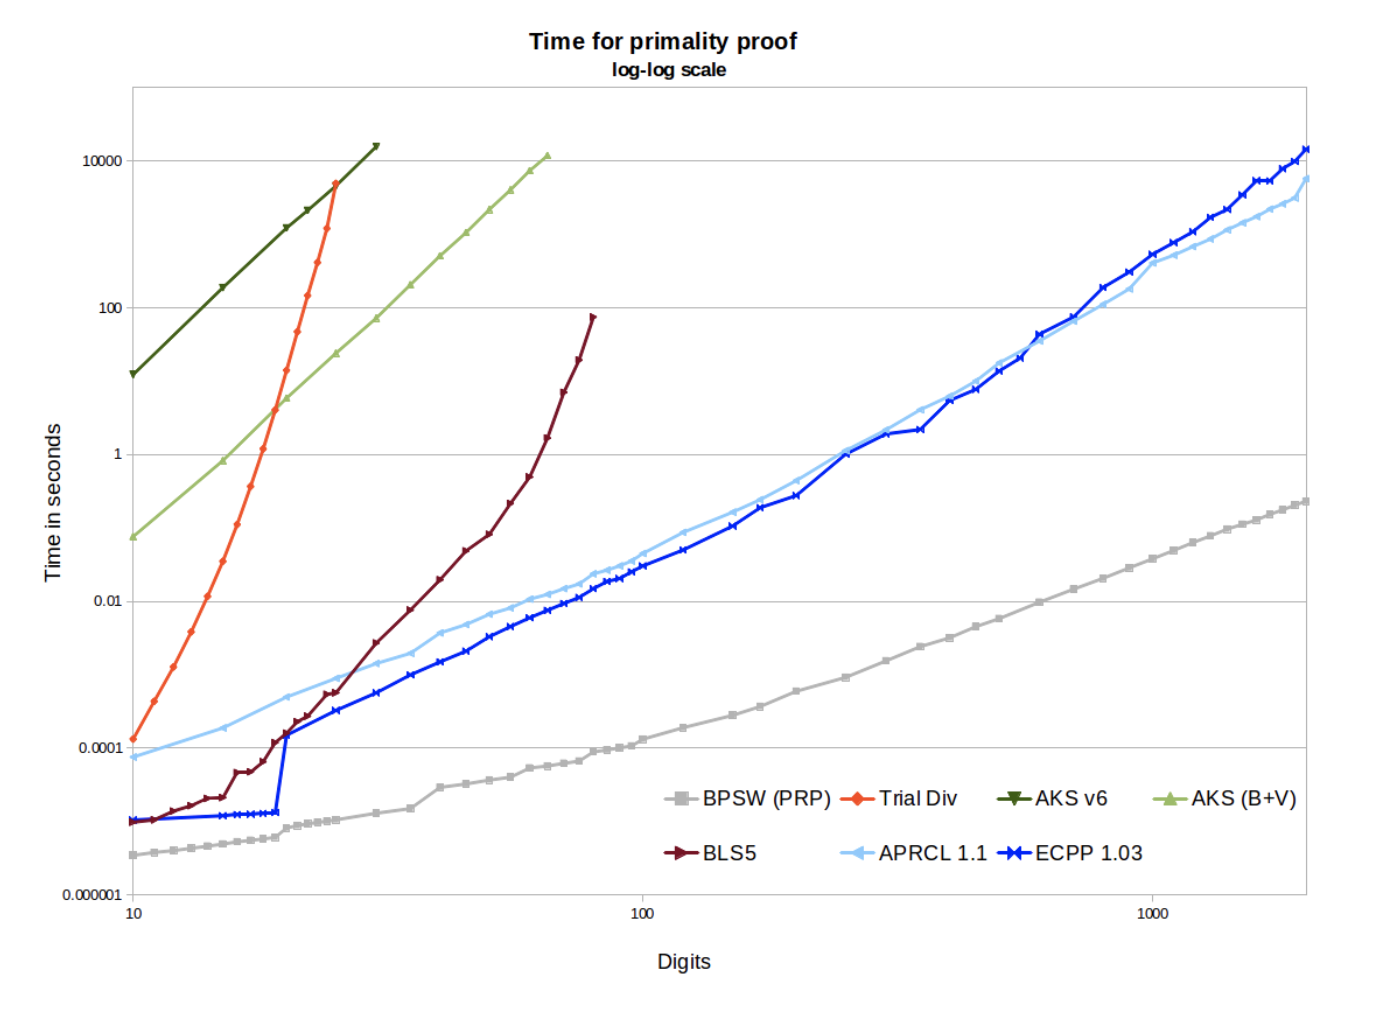
\includegraphics[width=13cm]{plots/Screenshot 2020-04-23 at 02.12.06.png}
\centering
\caption{\small{Laufzeit des AKS-Algorithmus im Vergleich zu anderen populären Primzahltests}}
\end{figure}

\newpage

\section{Experimentelle Auswertung}
In diesem Kapitel werden die Hauptschritte des AKS-Algorithmus(Schritt 2 und 5) untersucht, es wird unter anderem gezeigt, dass die Laufzeit dieser Schritte polynomiell von der Eingabegröße abhängig ist. Der Fokus liegt hier nicht auf die Korrektheit dieser Schritte(Dies wurde schon im 4. Kapitel gezeigt) sondern auf die polynomielle Laufzeit. Schließlich wird der AKS-Primzahltest mit dem naiven Primzahltest verglichen\footnote{. Der naive Algorithmus testet ob die eine Zahl $n$ einen Primfaktor $\leq  \sqrt{n}$ hat.}. 

Um dies illustrieren zu können, sind folgende Mengen erforderlich:
\begin{enumerate}
    \item \textbf{Menge 1:} Die Menge der Primzahlpotenzen.\newline
    $M_1 = \{ n \in \mathbb{N} \mid n = a^b, \, a \in \mathbb{P}, \, b \in \mathbb{N}\}$.\newline
    
    \item \textbf{Menge 2:} Die Menge aller Zahlen, die nicht aus der ersten Menge sind, aber zusammengesetzt sind. $M_2 = \{ n \in \mathbb{N}\setminus	 M_1 \mid 1 < (a,n) < n, \forall a \leq \sqrt{n} \}$.\newline
    
    \item \textbf{Menge 3:} Die Menge der Zahlen, die weder aus $M_1$ noch aus $M_2$, sodass die Gleichung \ref{eq:2}, die im 3 Kapitel beschrieben wurde, erfüllt ist. $M_3 = \{ n \in \mathbb{N} \setminus (M_1 \cup M_2) \mid \exists a,r : (X + a)^n \neq X^n + a \, (\, mod \, X^r - 1,p) \}$
\end{enumerate}



\subsection{Implementierungsdetails}
Zur Implementierung der Algorithmen wurde das Computer-Algebra System SageMath verwendet. Die Grafiken wurden mithilfe von der öffentlichen Library MatplotLib gemacht. Der Quellcode ist auf meinem Github: \url{https://github.com/salman13s/Bachelorarbeit} zu finden. Die Experimente wurden auf einem Computer mit einem Intel Core i7 mit vier Kernen, die jeweils auf 2,8 GHz getaktet sind, und mit 16GB Arbeitsspeicher unter Mac OS Catalina 10.15.3 ausgeführt.\footnote{$\,$ Alle Zeitmessungen wurden mit der Python-Funktion process\_time() gemessen.}

\subsection{Experimentelle Ergebnisse}

\subsubsection{Experiment 1: Die Suche nach einem geeigneten $r$}
Einer der Hauptschritte des AKS-Algorithmus ist der zweite Schritt. Im zweiten Schritt wird nach einem $r$ gesucht, sodass $o_r(n) > log^2 n$. Dies passiert durch ausprobieren von mehreren $r$ Werten. In Lemma \ref{limit_of_r} wurde gezeigt, dass dieses $r$ existiert, es wurde außerdem gezeigt, dass $r \leq log^5 n$. In diesem Experiment wird gezeigt, dass die Laufzeit des 2. Schritts polynomiell von der Eingabegröße abhängig ist.

\textbf{\samll{Beschreibung des Experiments:}}\newline
In diesem Experiment soll die polynomielle Laufzeit des zweiten Schritts vom AKS-Primzahltest demonstriert werden. Hierzu werden verschiedene Inputgrößen betrachtet. Für jede Inputgröße werden 100 zufällig ausgewählte Datenpunkte verwendet, danach wird für jeden Datenpunkt die Laufzeit gemessen. Dadurch erhält man mehrere verstreute Punkte im zweidimensional Raum. Nun wird ein Polynom an diese Punkte angepasst, dieses Polynom soll (Gemäß Kapitel 4) Grad 7 haben. Dafür sind folgende Mengen erforderlich:

\begin{enumerate}
    \item $I = \{ I_{1},I_{2}, \dots, I_{n} \}$ Menge der Inputs, die Inputs sind in diesem Fall Arrays von  Bitlängen. $I_{k}$ beschreibt die Menge der Zahlen, die Bitlänge $k$ haben\footnote{$I_{k} = \{ n \in \mathbb{N} \mid \lVert n\rVert = k\}$}\newline
    
    \item $ T = \{T_{1},T_{2}, \dots, T_{n}\}$ Menge der Outputs, hier sind die Outputs Arrays von gemessenen Laufzeiten für die jeweiligen Inputs.\newline 
    
    \item $T_{max} = \{ &max\{ T_{1} \},max\{ T_{2} \}, \dots, max \{ T_{n} \} \}$.\newline
    \item $I_{r} = \{ k \mid \, \forall  I_{k} \in I \}$
\end{enumerate}
Das Ziel ist eine bestmögliche Approximation(durch ein Polynom) für die Funktion $f(x) = y$ zu berechnen, wobei $x \in I_{k}$ und $y \in T_{k}, k = 1,2, \dots, n$.

\textbf{\small{Erwartetes Verhalten:}}\newline
Das angepasste Polynom soll die Mittelwerte von den 100 Punkten bei jeder Inputgröße nahezu perfekt darstellen.

\textbf{\small{Die Daten:}}
Für dieses Experiment wurden 14 Inputgrößen verwendet.\newline 
$I = \{ I_{8},I_{9},I_{10},I_{12},I_{13},I_{15},I_{16},I_{17},I_{19},I_{22},I_{24},I_{25},I_{27} \}$.

\textbf{\small{Ergebnisse:}}
\begin{figure}[h]
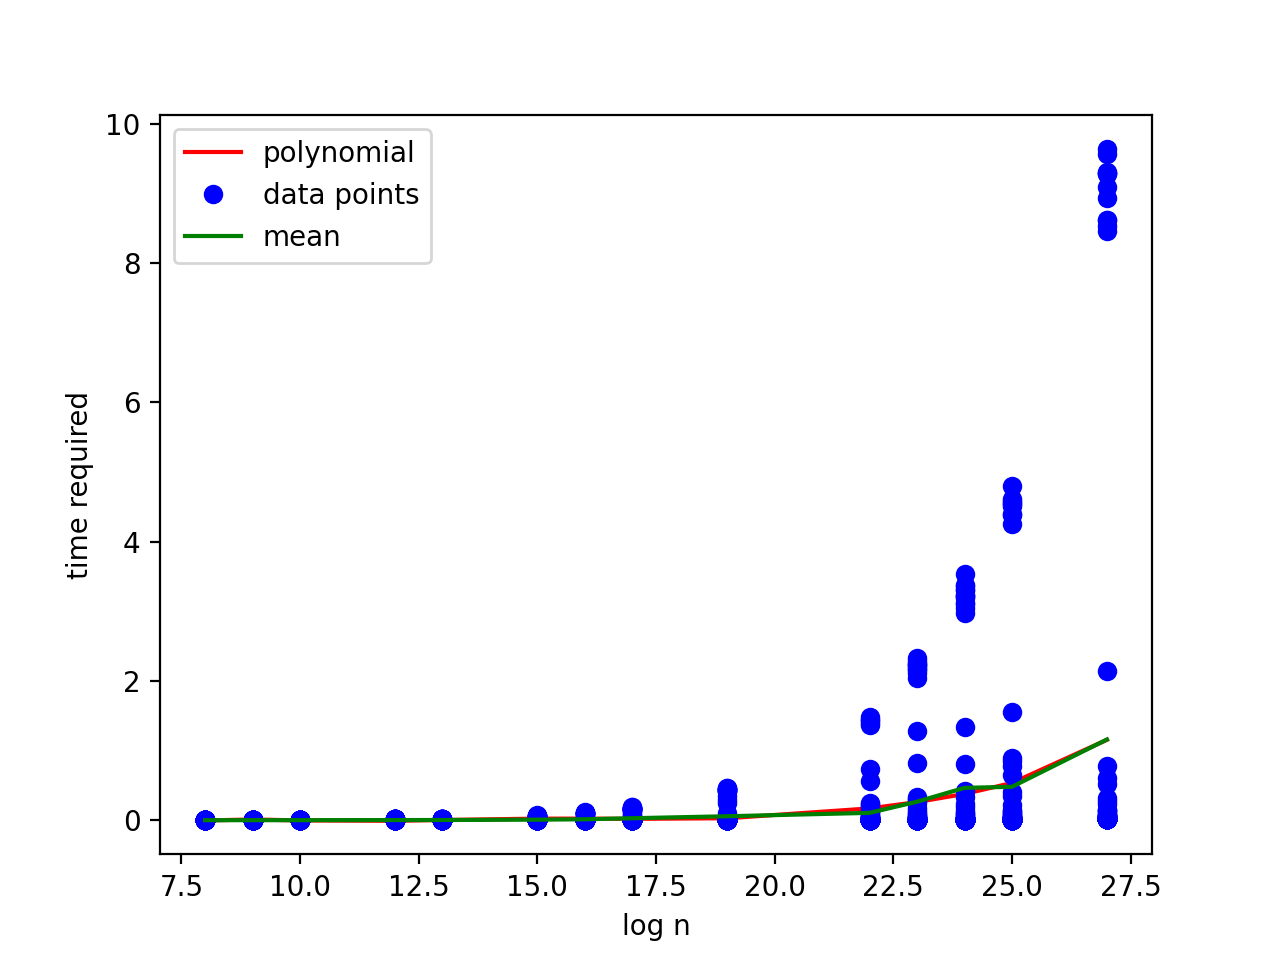
\includegraphics[width=10cm]{plots/runtime_find_r.png}
\centering
\caption{Anpassung des Polynoms an die Laufzeiten}
\label{runtime-find_r}
\end{figure}

Abbildung \ref{runtime-find_r} zeigt, dass das gewählte Polynom vom Grad 7 (rot) die Funktion der Mittelwerte von den Inputgrößen(grün) nahezu zu perfekt darstellt. Mit Hilfe dieser empirischen Evidenz kann man nun folgern, dass die Average-Case-Complexity $\Theta(t(n))$ polynomiell ist. Das heißt $\Theta^{\sim}(log^k  n), k > 0$. In diesem Fall ist $k = 7$.


Des Weiteren kann mit Hilfe dieser Datenpunkte auf ähnlicher Weise auch den schlechtmöglichsten Fall(Worst-case-Complexity) bestimmen. Hierzu wird das Polynom durch die Maximumpunkte von $T_{k}, \, k = 1,2, \dots, n$ angepasst.
Folgende Funktion wird nun approximiert: 
\begin{align*}
    f(x) = y, \, wobei \,y \in T_{max} , x \in I_{r}.
\end{align*}

\begin{figure}[h]
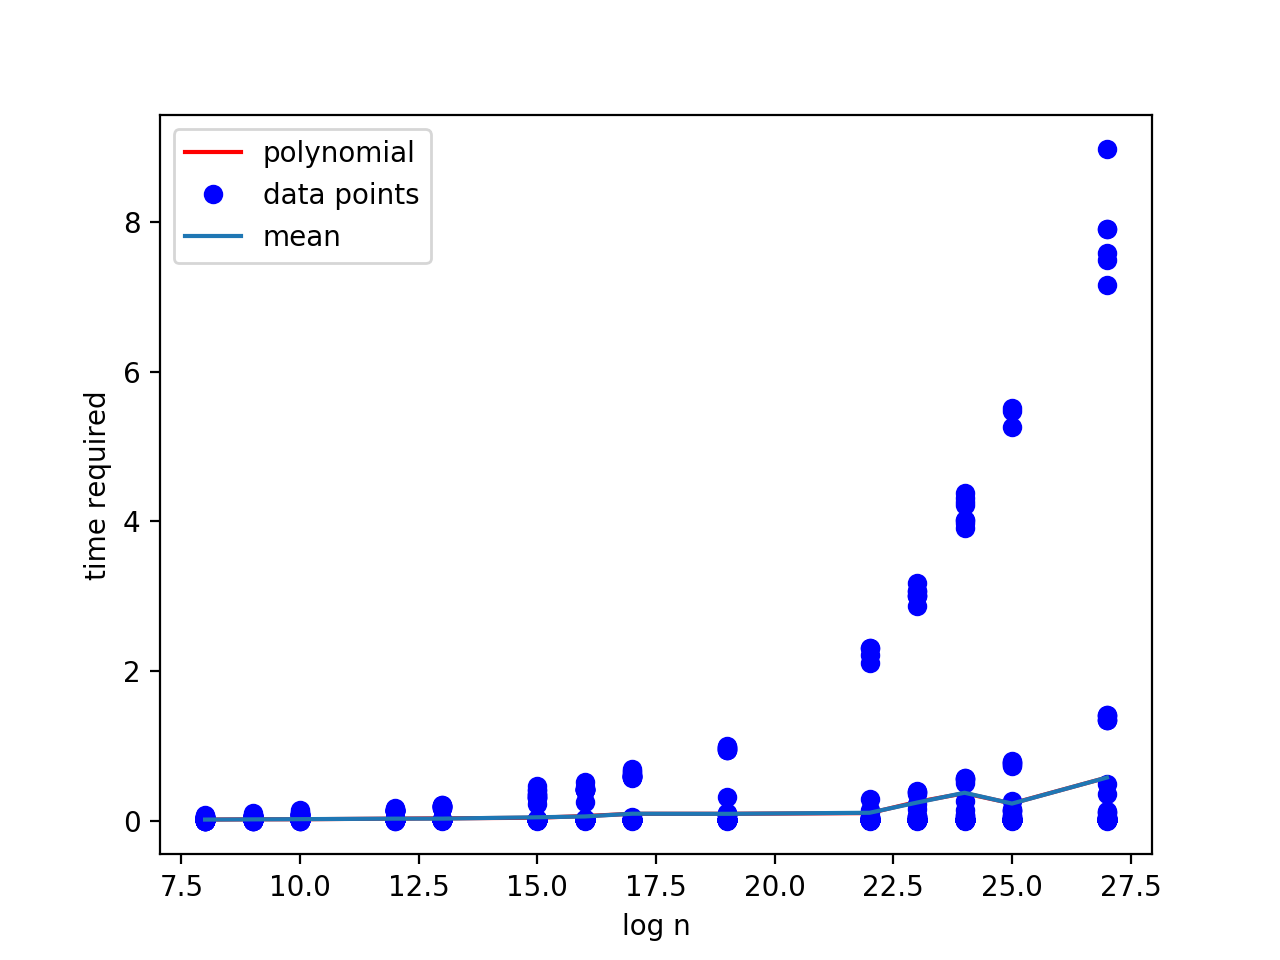
\includegraphics[width=10cm]{plots/aks_run_time.png}
\centering
\caption{Anpassung des Polynoms an die höchsten Laufzeiten}
\label{runtime-aks}
\end{figure}







\subsubsection{Experiment 2: Laufzeit des AKS-Algorithmus}
In diesem Experiment wurde die Laufzeit des AKS-Algorithmus für mehrere bekannte Primzahlen gemessen\footnote{$\,$ Für die Primzahlen siehe \url{http://compoasso.free.fr/primelistweb/page/prime/liste_online_en.php} und \url{https://en.wikipedia.org/wiki/Largest_known_prime_number}.}. Es wurden auch bekannte zusammengesetzte Zahlen eingegeben, um die Korrektheit des AKS-Algorithmus zu testen.
\begin{table}[h!]
\centering
\begin{tabular}{ |p{3cm}||p{3cm}|p{3cm}|p{3cm}|  }
 \hline
 \multicolumn{4}{|c|}{AKS-Algorithmus} \\
 \hline
 Zahl & Inputgröße &Ergebnis&Zeit in s\\
 \hline
 49   & 6    &False&   $8.5 \cdot 10^{-5}$\\
 233&   8  & True   &$0.063$\\
 12923 &14 & True&  $0.302$\\
 131071    &17 & True&  $1.006$\\
 3875741& 22  & True   &$2.9943$\\
 38890279& 26  & True& $7.890$\\
 2147483647&   31  & True& $43.54$\\
 90552556447&   37  & False& $18.781$\\
 140141183298&   38  & False& $0.019$\\
 147763360000&   38  & False& $0.000065$\\
 170141183297& 38 & True& $119.432$\\
 \hline
\end{tabular}

 \caption{Laufzeituntersuchung des AKS-Algorithmus.}
\label{table:3}
\end{table}

Man kann nun anhand der Primzahlen der obigen Tabelle eine Grafik plotten, um die Steigerung der Laufzeit zu verdeutlichen. 

\begin{figure}[h]
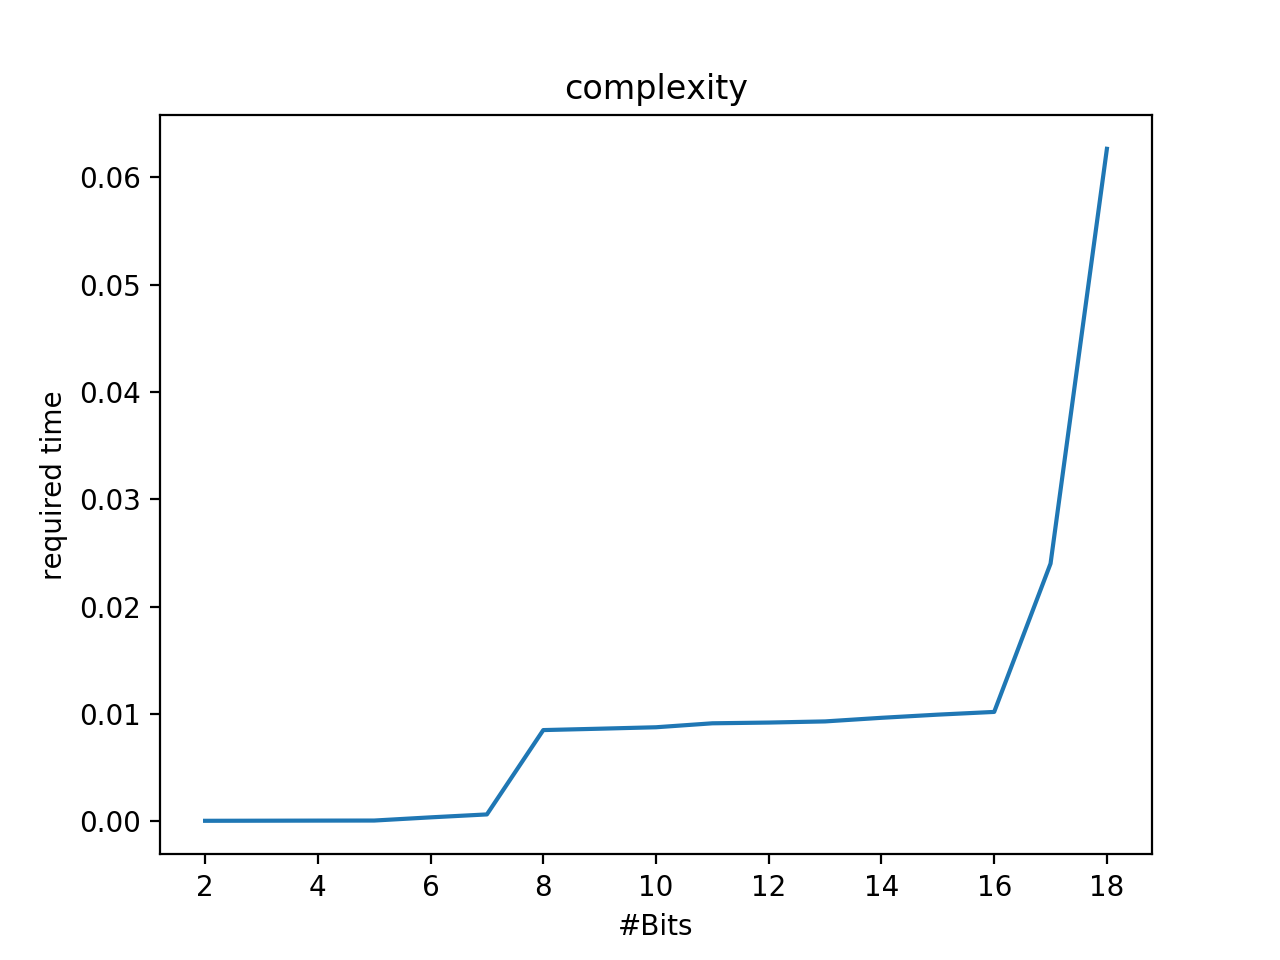
\includegraphics[width=7.06cm]{plots/aks.png}
\centering
\caption{Laufzeit des AKS-Primzahltests}
\label{aks-runtime}
\end{figure}



% TODO: rewrite the whole passage !!
Tabelle \ref{table:3} und Abbildung \ref{aks-runtime} zeigen deutlich, dass der zeitliche Aufwand des AKS-Algorithmus für Primzahlen kontinuierlich steigt, wenn die Eingabegröße größer wird. Das ist aber nicht unbedingt der Fall für zusammengesetzte Zahlen, da es zusammengesetzte Zahlen gibt, die schon im ersten Schritt des Algorithmus identifiziert werden, da sie Primzahlpotenzen sind. Ein Beispiel dafür wäre die Zahl 147763360000 mit der Inputgröße 38. Für diese Zahl hat der Algorithmus $6.5 \cdot 10^{-5}$ s gebraucht, und das ist wesentlich weniger als die gemessene Zeit für 90552556447 mit Inputgröße 37.


\subsubsection{Experiment 3: AKS vs naiver Primzahltest}
In der Einführung dieser Arbeit wurde ein Algorithmus(naiver Algorithmus) erwähnt, der das Primalitätsproblem in $\Omega(\sqrt{n})$ löst. Allerdings hat dieser Algorithmus eine exponentielle Laufzeit. Der AKS-Algorithmus hat eine polynomielle Laufzeit, und ist somit schneller als der naive Primzahltest(engl. brute-force primality test). In diesem Experiment wurden die Laufzeiten beider Algorithmen bis zur Inputgröße $37$ verglichen.  

Zur Untersuchung der Laufzeit beider Algorithmen als Primzahltest werden bewusst nur Primzahlen als Eingabewerte herangezogen. Das liegt einerseits daran, dass diese den schlechtest möglichen Fall beider Algorithmen darstellt. Andererseits ist oft der Fall, dass der AKS-Algorithmus für zusammengesetzte Zahlen aus $M_1$ das Ergebnis  schnell liefern kann.\footnote{. Dadurch soll ein Verglich zwischen der Potenz-Prüfung und dem naiven Algorithmus vermieden werden.}\newline

Der naive Primzahltest hat eine exponentielle Laufzeit, das heißt aber nicht, dass der naive Algorithmus für alle Inputgrößen langsamer als der AKS-Algorithmus ist. Es kann sein, dass der naive Algorithmus z.B. für kleine Inputgrößen eine schnellere Antwort als der AKS-Algorithmus liefert. Folgende Tabelle ist einerseits ein sehr schönes Beispiel für die immense Steigerung der Laufzeit des naiven Primzahltests. Andererseits ist sie auch ein Beispiel für den Fall, wo der naive Algorithmus schneller als der AKS-Algorithmus ist. 
\begin{table}[h!]
\centering
\begin{tabular}{ |p{3cm}||p{3cm}|p{3cm}|p{3cm}|  }
 \hline
 \multicolumn{4}{|c|}{AKS vs Naive} \\
 \hline
 Zahl & Inputgröße  & AKS [in s] &Naive [ in s]\\
 \hline
 8191   & 13    &0.319566&   0.0006\\
 131071&   17  & 0.990821   &0.01\\
 524287 &19 &  1.5811& 0.04\\
 38757413    &26 & 7.556&   2.933\\
 2147483647& 31  & 42.58   &162.3\\
 2547587681& 32  &  43.902&  187.876\\
 17014120163&   34  & 86.073& 1275.286\\
 90552556889&   37  & 97.769072& 6732.12\\

 \hline
\end{tabular}
 \caption{AKS vs naiver Primzahltest.}
\label{table:4}
\end{table}



Obige Tabelle macht auch deutlich, dass der AKS-Algorithmus eine bessere asymptotische Laufzeit als der naive Algorithmus hat. Es ist aber augenfällig, dass der AKS-Algorithmus für Inputgrößen kleiner gleich 26 langsamer als der naive Algorithmus ist. Das liegt daran, dass die Laufzeit des AKS-Algorithmus $O^{\sim}(log^{10.5}n)$ beziehungsweise $O^{\sim}(log^7n)$(wenn $n \leq r$) für "kleine" $ $ Inputgrößen größer oder gleich als die Laufzeit des naiven Algorithmus $O(\sqrt{n})$ ist. Dies lässt sich am besten durch eine Grafik illustrieren. 


\begin{figure}[h]
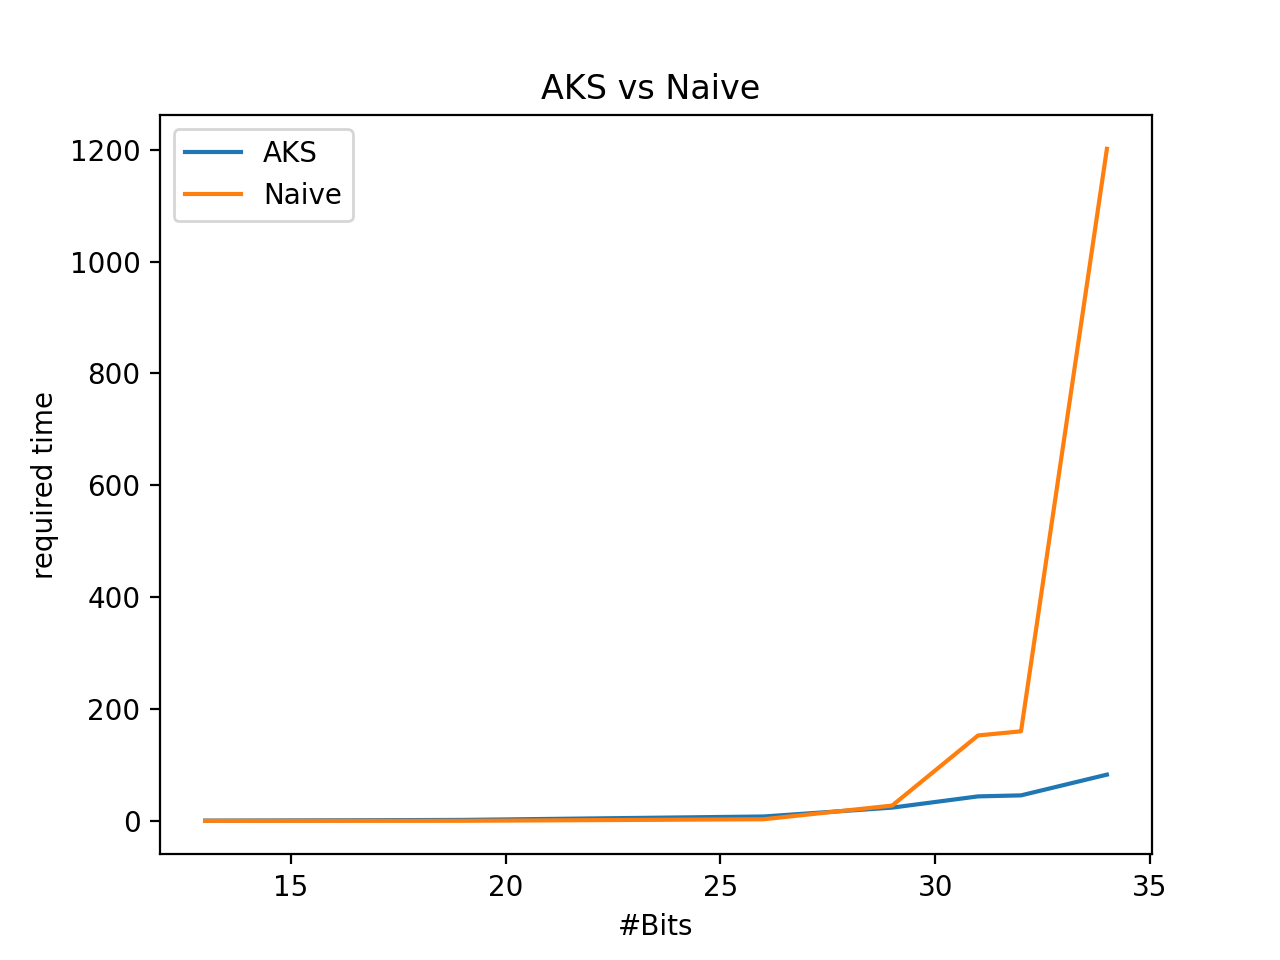
\includegraphics[width=8cm]{plots/aksVsNaive.png}
\centering
\caption{Laufzeit des AKS-Algorithmus im Vergleich zum naiven Algorithmus}
\label{plot_aks_naive}
\end{figure}

In der Grafik \ref{plot_aks_naive} sieht man, dass der AKS-Algorithmus bei Inputgröße $37$ in unter $200 \, s$ eine Antwort geliefert hat, während der naive Algorithmus mehr als $6500 \, s(> 1.5 h)$ brauchte.\footnote{In der Tabelle wurde die Laufzeit von Zahlen bis Inputgröße 37 gemessen, während in der Grafik nur Zahlen mit Inputgröße bis 35 zu sehen sind. Das liegt  einerseits daran, dass die Grafik für diese Werte übersichtlicher ist. Andererseits sind diese ausreichend, um zu zeigen, dass die Laufzeit des AKS-Algorithmus wesentlich besser ist.} Aber bei Inputgrößen bis ungefähr 29 ist die Laufzeit beider Algorithmen fast identisch. Das heißt, der AKS-Algorithmus hat eine bessere asymptotische Laufzeit. 

\newpage

\section{Zusammenfassung}
Zur Anfang der Arbeit wurde der Stand vom Primalitätstesten vor dem AKS-Algorithmus kurz dargestellt. Danach wurden der AKS-Algorithmus und seine Grunde im Detail beschrieben. Hierzu gehörte unter anderem die Identität, auf der der AKS-Primzahltest aufbaut. Diese Identität war der Ausgangspunkt dieser Arbeit. Zuerst wurden bestimmte Anforderungen für die Variablen $a,r$ Vorausgesetzt, die unbedingt für die Polynomiallaufzeit des AKS-Algorithmus erforderlich sind. Aus diesen Voraussetzungen wurde eine obere Schranke für die Anzahl der zu testenden $a$ Werte hergeleitet.

Nach der Vorstellung des AKS-Algorithmus und seine nötigen Voraussetzungen wurde der Korrektheitsbeweis durchgeführt. Im Beweis wurde gezeigt, dass der Algorithmus als ein Primzahltest verwendet werden kann, das heißt der Algorithmus liefert stets 1 (PRIME), wenn die Eingabe $n$ eine Primzahl ist. Aber auch wenn die Ausgabe 1 (PRIME) ist, dann ist die eingegebene Zahl $n$ tatsächlich eine Primzahl.

Nachdem die Korrektheit des Algorithmus bewiesen wurde, wurde die Laufzeitanalyse dargestellt. Zunächst wurde eine Abschätzung für das $r$ gemacht und mit Hilfe dieser Abschätzung wurde die Laufzeitanalyse durchgeführt. Diese Analyse ergab, dass der Algorithmus eine polynomielle Laufzeit hat. Es wurden außerdem mehrere Verbesserungen für die Laufzeit vorgeschlagen. Einige Verbesserungen waren auf Vermutungen basiert. Es gab aber auch einen anderen Ansatz mit dem sich die Laufzeit $O^{\sim}(log^{10.5}n)$, ohne auf Vermutungen zurückgreifen zu müssen auf $O^{\sim}(log^6n)$ reduzieren lässt. Im gleichen Kapitel wurde kurz diskutiert, warum der AKS-Algorithmus nicht in der Praxis einsetzbar ist.

Es wurde auch mit Hilfe von mehreren Experimenten demonstriert, dass der AKS-Algorithmus korrekt ist und darüber hinaus eine polynomielle Laufzeit hat. Schließlich wurde der AKS-Algorithmus mit dem naiven Algorithmus --der Probedivision Algorithmus-- verglichen. Dadurch hat sich herausgestellt, dass der AKS-Algorithmus eine bessere asymptotische Laufzeit hat.

Der AKS-Primzahltest ist ein wichtiger theoretischer Durchbruch im Bereich der Primalitätstesten, er war der erste deterministische bedingungslose Algorithmus mit polynomielle Laufzeit. Aber in der Tat ist der Algorithmus Trotz seiner Eigenschaften immer noch für große Primzahlen sehr langsam\footnote{Die größte bekannte Primzahl $2^{82589933} - 1$ hat $24862048$ Stellen.}. Daher wird weder der AKS-Algorithmus noch seine randomisierte Version in der Praxis benutzt\cite{mit_aks}.



 


%%%%%%%%%%%%%%%%%%%%%%%%%%%%
%% Literaturverzeichnis wird 
%% automatisch eingefügt
%%%%%%%%%%%%%%%%%%%%%%%%%%%%
\clearpage
\lhead{}
\printbibliography
\addcontentsline{toc}{section}{\bibname}


%%%%%%%%%%%%%%%%%%%%%%%%%%%%
%% Anhang (optional) 
%%%%%%%%%%%%%%%%%%%%%%%%%%%%
\clearpage
\appendix
\section{Algorithmenverzeichnis}
% check_perefect_powers
\begin{algorithm}[H]
\SetAlgoLined
\KwIn{$n \in \mathbb{N}, n \geq 2$.}
\begin{enumerate}
\item $a, \, b, \, c, \, m$

\item $ b = 2$.

\item \textbf{while} $2^b \leq n$ \textbf{repeat}

\item $\: \: \: \: $ $a = 1, \, c = n $

\item $\: \: \: \: $ \textbf{while} $c - a \geq 2$ \textbf{repeat}

\item $\: \: \: \: \: \: \: \: \:$ $ m = \lfloor (a + c)/2 \rfloor$

\item $\: \: \: \: \: \: \: \: \:$ $ p = min\{m^b,n+1\}$

\item $\: \: \: \: \: \: \: \: \:$ \textbf{if} $ p = n$ \textbf{return} True.

\item $\: \: \: \: \: \: \: \: \:$ \textbf{if} $p < n$

\item $\: \: \: \: \: \: \: \: \: \: \: \: \: \:$  $ a = m$

\item $\: \: \: \: \: \: \: \: \:$ \textbf{else}

\item $\: \: \: \: \: \: \: \: \: \: \: \: \: \:$  $c = m$

\item $\: \: \: \: $ $b = b + 1$

\item \textbf{return} False


\end{enumerate}
\caption{Potenz-Prüfung}
\label{appendix:potenz}
\end{algorithm}

% fast expo algorithm
\begin{algorithm}[H]
\SetAlgoLined
\KwIn{$a \in M, n \geq 0$}
\begin{enumerate}
    \item $u = n$.
    \item $s = a$.
    \item $c = 1$.
    \item \textbf{while} $u \geq 1$ \textbf{repeat}
    \item $\; \: \: \;$ \textbf{if} $u \, mod \, 2 \neq 0$ \textbf{then}
       $ \; c = c \circ s$
     \item $\; \: \: \;$ $s = s \cdot \, mod \, M$
     \item $\; \: \: \;$ $ u = u \, div \, 2$
     \item \textbf{return $c$}
\end{enumerate}
 \caption{Schnelle modulare Exponentiation}
 \label{appendix:fast_expo}
\end{algorithm}

%%%%%%%%%%%%%%%%%%%%%%%%%%%%
%% Eidesstattliche Erklärung
%% muss angepasst werden 
%% in Erklaerung.tex
%%%%%%%%%%%%%%%%%%%%%%%%%%%%
\newpage
\begin{otherlanguage}{ngerman}
\thispagestyle{empty}
\section*{Eidesstattliche Erklärung}
\thispagestyle{empty}
Hiermit versichere ich, die vorliegende Arbeit selbstständig verfasst und keine anderen als die angegebenen Quellen und Hilfsmittel benutzt sowie die Zitate deutlich kenntlich gemacht zu haben.
\newline
\vspace{4\baselineskip}\\
Leipzig, den \today \hfill Salman Salman 
\vspace{4\baselineskip}\\
\end{otherlanguage}

\end{document}
